\documentclass{sig-alternate}
\usepackage[utf8]{inputenc}
\usepackage{times}
\usepackage{gensymb}
\usepackage{epsfig}
\usepackage{xcolor}
\usepackage{xspace}
\usepackage{multicol}
\usepackage{listings}
\usepackage{verbatim}
\usepackage{hyperref}
\usepackage{caption}
\usepackage{subcaption}

\usepackage[protrusion=true,expansion=true]{microtype}
\setlength{\emergencystretch}{3em}



\begin{document}
\conferenceinfo{CIDR '17}{January 8-11, 2017, Chaminade, CA, USA}
\newcommand{\smallitem}[1]{\vspace{0.5em}\noindent\textbf{#1}}
\newcommand{\smallitembot}{\vspace{0.5em}\noindent}
\bibliographystyle{abbrv}

% \newcommand{\jmh}[1]{{\textcolor{red}{[[#1 -- jmh]]}}}
% \newcommand{\joey}[1]{{\textcolor{cyan}{[[#1 -- jeg]]}}}
% \newcommand{\msd}[1]{{\textcolor{green}{[[#1 -- msd]]}}}
% \newcommand{\akon}[1]{{\textcolor{orange}{[[#1 -- akon]]}}}
% \newcommand{\vikram}[1]{{\textcolor{blue}{[[#1 --vikram]]}}}
\newcommand{\jmh}[1]{}
\newcommand{\joey}[1]{}
\newcommand{\msd}[1]{}
\newcommand{\akon}[1]{}
\newcommand{\vikram}[1]{}

% \newcommand{\cab}{CAB\xspace}
\newcommand{\core}{version graph\xspace}
\newcommand{\mantle}{model graph\xspace}
\newcommand{\crust}{lineage graph\xspace}
\newcommand{\Core}{Version Graph\xspace}
\newcommand{\Mantle}{Model Graph\xspace}
\newcommand{\Crust}{Lineage Graph\xspace}

\newcommand{\version}{\kw{Version}\xspace}
\newcommand{\richversion}{\kw{RichVersion}\xspace}
\newcommand{\thing}{\kw{Item}\xspace}
\newcommand{\GroundItem}{\kw{Item}\xspace}
\newcommand{\node}{\kw{Node}\xspace}
\newcommand{\edge}{\kw{Edge}\xspace}
\newcommand{\structure}{\kw{Structure}\xspace}
\newcommand{\graph}{\kw{Graph}\xspace}
\newcommand{\TVID}{\kw{TVID}\xspace}
\newcommand{\gtag}{\kw{Tag}\xspace}
\newcommand{\uri}{\kw{URI}\xspace}

\newcommand{\versiongraph}{versiongraph\xspace}
\newcommand{\modelgraph}{modelgraph\xspace}
\newcommand{\lineagegraph}{lineagegraph\xspace}
\newcommand{\versiongraphs}{versiongraphs\xspace}
\newcommand{\modelgraphs}{modelgraphs\xspace}
\newcommand{\lineagegraphs}{lineagegraphs\xspace}
\newcommand{\groundwire}{GroundWire\xspace}

\newcommand{\kw}[1]{{\small\texttt{#1}}}
\newcommand{\lilemail}[1]{\email{\small #1}}



\title{Establishing Common Ground with Data Context}
% \title{Grounding Data Context Through Big Metadata  }
% \title{Grounding Big Data with Data Context Services}

\numberofauthors{1}
\author{
\alignauthor
Joseph M.\ Hellerstein\textsuperscript{*}, 
Vikram Sreekanti\textsuperscript{*}, 
Joseph E. Gonzalez\textsuperscript{*},
Sudhanshu Arora\textsuperscript{$\ddagger$},
Arka Bhattacharyya\textsuperscript{*},
Shirshanka Das\textsuperscript{$\dagger$}, 
Akon Dey\textsuperscript{$\sharp$}, 
Mark Donsky\textsuperscript{$\ddagger$}, 
Gabriel Fierro\textsuperscript{*},
Sreyashi Nag\textsuperscript{$\S$}, 
Krishna Ramachandran\textsuperscript{$\natural$}, 
Chang She\textsuperscript{$\ddagger$},
Eric Sun\textsuperscript{$\dagger$}, 
Carl Steinbach\textsuperscript{$\dagger$}
Venkat Subramanian\textsuperscript{$\flat$}\\
{\small
\textsuperscript{*}UC Berkeley, 
\textsuperscript{$\ddagger$}Cloudera,
\textsuperscript{$\dagger$}LinkedIn,
\textsuperscript{$\sharp$}Awake Networks,
\textsuperscript{$\S$}University of Delhi,
\textsuperscript{$\natural$}Skyhigh Networks,
\textsuperscript{$\flat$}Dataguise
}
}

% \numberofauthors{8}
% \author{
% % 1st. author
% \alignauthor
% Joseph M.\ Hellerstein\\
%       \affaddr{Berkeley}\\
%       \lilemail{AuthorEmail@gmail.com}
% % 2nd. author
% \alignauthor
% Vikram Sreekanti\\
%       \affaddr{Berkeley}\\
%       \lilemail{AuthorEmail@gmail.com}
% % 3rd. author
% \alignauthor
% Joseph E. Gonzalez\\
%       \affaddr{Berkeley}\\
%       \lilemail{AuthorEmail@gmail.com}
% \and  % use '\and' if you need 'another row' of author names
% % 4th. author
% \alignauthor
% Akon Dey\\
%       \affaddr{Awake Networks}\\
%       \lilemail{AuthorEmail@gmail.com}
% % 5th. author
% \alignauthor
% Mark Donsky\\
%       \affaddr{Cloudera}\\
%       \lilemail{AuthorEmail@gmail.com}
% % 6th. author
% \alignauthor
% Sreyashi Nag\\
%       \affaddr{University of Delhi}\\
%       \lilemail{AuthorEmail@gmail.com}
% \and
% \alignauthor
% Krishna Ramchandran\\
%     \affaddr{FICO}\\
%     \lilemail{AuthorEmail@gmail.com}
% \alignauthor
% Chang She\\
%     \affaddr{Cloudera}\\
%     \lilemail{AuthorEmail@gmail.com}
% \alignauthor
% Carl Steinbach\\
%     \affaddr{LinkedIn}\\
%     \lilemail{AuthorEmail@gmail.com}
% }


\maketitle

% \joey{original abstract}
\begin{abstract}
Ground is an open-source \emph{data context service}; a system to manage all the peripheral information that informs the use of data. 
% \joey{I know we keep referring to the technology as a service but perhaps the paper should refer to it as a framework?}
Data usage has changed both philosophically and practically in the last decade, creating an opportunity for new data context services to foster further innovation.
In this paper we frame the challenges of managing data context along three axes: \emph{Applications}, \emph{Behavior}, and \emph{Change}. 
We provide motivation and design guidelines, present our initial design of a common metamodel and API, and explore the current state of the storage solutions that could serve the needs of a data context service. 
Throughout, we highlight opportunities for new research and engineering solutions.
\end{abstract}

% \begin{abstract}
% % % The disaggregation of data systems has fostered substantial growth in data technologies and enabled organizations to be more agile in how they store, manage, and use data.
% % % Data systems today are addressing significant changes in usage, shifting from tightly-controlled
% % % data warehouses to agile and exploratory data lake projects. Along with these changes
% % % comes a change in te soft
% % Typically usage of databases has shifted in recent years, from tightly-controlled
% % data warehouses to open-ended data lakes with many users and applications.
% % Meanwhile, modern data systems have shifted to decoupled designs, in traditionally
% % tightly-coupled systems are provided as independent, swappable components
% % with standard APIs. These changes present an
% % % However the movement towards 
% % % % more fluid, 
% % % disaggregated
% % % % , and highly agile 
% % % data systems presents an 
% % Over the last decade, data has become a central resource for most organizations, with a growing set of stakeholders. Technologists have responded to this diversity of interest with new work practices and software, which have accelerated these
% % trends. These rapid changes bring with them an
% % existential % joey -- ok this might be a bit dramatic but ...
% % challenge: how do we manage \emph{data context} in an increasingly decoupled and diverse world?
% % The interpretation of data, its change history and its usage
% % % , how it is being used, who is using it, and for what purposes --- is essential to both maximizing the value of data and also minimizing the risk. 
% % all provide critical information typically lost in modern organizations.
% % Data context is often more challenging to manage than data itself, encompassing data and usage, spanning multiple systems, and sometimes growing larger than the underlying data.

% % Take credit for framing the problem!
% % Take credit for proposing a solution 
% Using these axes we introduce Ground: an open-source \emph{data context service} to manage all the peripheral information that informs the use of data. 
% % Describe how solution connects to framing
% We describe an early prototype of Ground that exposes a narrow waist context service built on flexible metamodel. 
% We present early experimental results on our prototype implementation of Ground and outline emerging technical challenges.
% % both above and below Ground.
% % \joey{We need one sentence connecting solution to framing and highlighting the big design idea in Ground.}
% % \joey{We need one sentence describing earl results and applications.}
% \end{abstract}







\section{From Crisis to Opportunity}
Traditional database management systems were developed in an era of risk-averse design.
The technology itself was expensive, as was the on-site cost of managing it. Expertise
was scarce and concentrated in a handful of computing and consulting firms.

Two conservative design patterns emerged that lasted many decades. First, the accepted best practices
for deploying databases revolved around tight control of schemas and data ingest in support of 
general-purpose accounting and compliance use cases. 
Typical advice from data
warehousing leaders held that 
\emph{``There is no point in 
bringing data $\ldots$ into the data warehouse environment without integrating it.''}~\cite{inmon2005building} 
Second, 
the data management systems designed for these users were often built by a single vendor and deployed as a
monolithic stack. % spanning data ingest, storage, retrieval, and governance.
% regardless of how well-factored they were under the covers. %\msd{Although} 
A traditional DBMS included a consistent storage engine, a dataflow engine, 
a language compiler and optimizer, a runtime scheduler, a metadata catalog, and facilities for data ingest 
and queueing---all designed to work closely together.


As computing and data have become orders of magnitude more efficient, changes have emerged for both of these patterns. 
Usage is changing profoundly, as expertise and control shifts from the central accountancy of an IT department to 
the domain expertise of ``business units'' tasked with extracting value from data~\cite{gartner}. 
The changes in economics and usage brought on the ``three V's'' of Big Data: Volume, Velocity and Variety.
Resulting best practices focus on open-ended schema-on-use
data ``lakes'' and agile development, in support of exploratory analytics and innovative application intelligence~\cite{patil2012data}. 
Second, while many pieces of systems software that have emerged in this space are familiar, the overriding architecture is profoundly 
different. In today's leading open source
data management stacks, nearly all of the components 
of a traditional DBMS are explicitly independent 
and interchangeable.  This architectural decoupling is 
a critical and under-appreciated aspect of the Big Data movement,
% swappable, with multiple choices in wide use today. 
enabling more rapid innovation and specialization.



% \vikram{Like we talked about yesterday, should we flip this and talk about the traditional database stack instead of introducing big data first?}\akon{I think so too. It is widely accepted that traditional systems handle this well. However, this is not just a Big Data issue.}
% % \joey{I see where everyone is coming from but I think the story is stronger if we focus on the limitations of data management in the ``big data''/``data lake'' worlds.}
% The open-source Big Data movement, spearheaded by Hadoop, is often discussed in terms of changes in usage. This includes the ``three V's'' of Volume, Velocity and Variety of data being captured, and the agile working style typified by ``schema-on-use'' and a wide diversity programming models.

% % Much less widely discussed is a 
% A driving force behind this proliferation of Big Data technologies is the
% % profound 
% shift towards highly decoupled data systems. 
% Traditionally, data systems were often designed by a single vendor and deployed as monolithic stacks spanning data ingest, storage, retrieval, and governance.
% % regardless of how well-factored they were under the covers. %\msd{Although} 
% A traditional DBMS included a consistent storage engine, a metadata catalog, a dataflow engine, a language compiler and optimizer, an execution scheduler/runtime, and facilities for data ingest and queueing all designed to work closely together.
%  %\msd{, it was simply seen as a DBMS}. 
% By contrast, in today's Big Data stack, nearly all of these components are explicitly independent and interchangeable with very narrow APIs.
% % swappable, with multiple choices in wide use today. 
% This decoupled architecture has enabled substantial innovation and specialization by fostering competition both in technology and price.
% % specialization 
% % % driving much of the excitement around big-data, 
% % and has been embraced by both developers and customers.

\subsection{Crisis: Big Metadata}

An unfortunate consequence of the disaggregated nature of contemporary data systems
% architecture
% One negative side-effect of this diversity
is the lack of a standard mechanism
% for shared metadata 
%\msd{metadata or data context?} 
% for these independently designed components 
to assemble a collective understanding of the origin, scope, and usage of the data they manage.
% metadata ``signature'' or ``paper trail'' of their content and behavior.
In the absence of a better solution to this pressing need,
% The current best solution to this pressing need 
% The only widely-deployed option 
% is the 
the 
Hive Metastore is sometimes used, but it only serves simple relational schemas---a dead end for representing a Variety of data. 
As a result, data lake projects typically lack 
even the most rudimentary information about the data they contain or how it is being used. 
% their components' behavior.
% ; it is often not even possible to discover what is being stored, much less how to manage it intelligently. 
For emerging Big Data customers and vendors, this \emph{Big Metadata} problem is hitting a crisis point.  

Two significant classes of end-user problems follow directly from the absence of shared metadata services.
%\jmh{Funny transition from software stack problem to usage problem. Need to start with interoperability and grow from there, or change preceding paragraph to focus on usage not the stack.}
%\joey{What are the problems? Could we introduce the ``Vs'' of metadata management: Discovery, Provenance, Attribution, Context ..., if we could articulate these clearly then we could perhaps translate their implications on administration, loss-of-value, risk to organization, ... }
The first is poor productivity.
%The promise of the Data Lake is that a diversity of data can be easily captured, and then harnessed by analysts for value. 
% In the absence of metadata,
Analysts are often unable to discover what data exists, much less how it has been previously used by peers. 
Valuable data is left unused
% opaque, 
and human effort is routinely duplicated---particularly in a schema-on-use world with raw data that requires preparation.  
% for use.
``Tribal knowledge'' is a common description for how organizations manage this productivity problem. 
This is clearly not a systematic solution, and scales very poorly as organizations grow.

The second problem 
stemming from the absence of a system to track metadata 
is governance risk. 
Data management necessarily entails tracking or controlling who accesses data, what they do with it, where they put it, and how it gets consumed downstream. 
%In some cases this governance metadata is used to enforce policy (e.g.\ access control for Personally Identifiable Information); in others it is logged to support audits for compliance (e.g.\ in the Basel Committee on Banking Supervision). 
In the absence of a standard place to store metadata and answer these questions, it is impossible to enforce policies and/or audit behavior. 
As a result, many administrators marginalize their Big Data stack as a playpen for non-critical data, and thereby inhibit both the adoption and the potential of new technologies.

% In our diverse experiences in industry, the authors 
% \joey{I think we should drop this paragraph.  This paragraph is only our personal assessment of our credibility which is hard to trust.}\jmh{I dunno, the reason we have so many people on this paper is because we've seen this problem in the field. Thoughts on how to word it differently but make that point?}\joey{Fine! it's not a bad paragraph and if we keep the big author list its compelling.}

In our experiences deploying and managing systems in production, we 
have seen the need for a common service layer to support the capture, publishing and sharing of metadata information in a flexible way. 
The effort in this paper began by addressing that need.

\subsection{Opportunity: Data Context}
\jmh{would be nice to weave agility in more aggressively}
The lack of metadata services in the Big Data stack can be viewed as an opportunity:
% is both a modern crisis
% but also an 
% clean-slate 
a clean slate to rethink how we track and leverage modern usage of data.
Storage economics and schema-on-use agility suggest that the Data Lake movement could go much farther than Data Warehousing in enabling diverse, widely-used central repositories of data that can adapt to new data formats and rapidly changing organizations.
In that spirit, we advocate rethinking traditional metadata in a far more comprehensive sense. 
More generally, what we should strive to capture is the full context of data.

To emphasize the conceptual shifts of this \emph{data context}, and as a complement to the ``three V's'' of Big Data,
we introduce three key sources of information---the \textbf{ABCs of Data Context}. Each represents a major change from the simple metadata of traditional enterprise data management.

% \msd{not sure where some of these metadata items would fit in: (1) business metadata (keywords, classification, compliance details, end-user tags), (2) operational metadata (date and execution details), (3) etc. - perhaps a bullet point list of the types of metadata and how it fits into ABC categories might help. I'm not sure that ABC covers the full scope.
% }
% \jmh{Took a crack at making sure these could fit in. See discussion after the list about whether to be explicit here.}

% \jmh{Want to make sure that we get each of A, B and C to have simple stories about what's novel. Right now it's in notes; ideally we find a paragraph structure where it fits into each paragraph neatly. Or we could have a separate table...}

% \vikram{``Change context'' sounds weird to me. Instead of calling each one context, can we say the ABCs of data context are application metadata, behavior and usage, and change over time? (or something like that). NOTE: Tentatively changing them. Leaving this here if we want to change back.} 
% \jmh{The words have to be as repeatable as the mnemonic that reminds us. We want lots of people to say ``The ABCs of Context: Axxx, Byyy and Czzz''. So one word each!}

\smallitem{Applications}: Application context is the core information that describes how raw bits get interpreted for use. 
In modern agile scenarios, application context is often relativistic (many schemas for the same data) and complex (with custom code for data interpretation). 
Application context ranges from basic data descriptions (encodings, schemas, ontologies, tags), to statistical models and parameters, to user annotations.  
%Application context today is often bespoke, specific to a single use case or set of use cases. But some application context is intended to be universally applied; e.g., access control or privacy information. Note that the interpretation of raw data typically requires executing code. 
All of the artifacts involved---transformation scripts, view definitions, model parameters, training sets, etc.---are critical aspects of application context. 
%\jmh{Novelties: subjectivity of models, inclusion of richer detail including code.}
% Application context includes both metadata and code.

\smallitem{Behavior}: This is information about how data was created and used over time. 
In decoupled systems, behavioral context spans multiple services, applications and formats and often originates from high-volume sources (e.g., machine-generated logs and sensors).
% It comes from a diverse set of applications, languages and compute frameworks, varying in granularity and interpretability.
Not only must we track upstream lineage---
% of a particular data object: 
the data sets and code that led to the creation of the data object---but we must also track the 
% It includes any
downstream lineage, including the data products that were derived from this data object. 
Aside from data lineage, behavioral context includes logs of usage: the ``digital exhaust'' left behind by computations on the data. 
As a result, behavioral context metadata can 
% grow to be extremely large: often 
often be larger than the data itself. 
% \jmh{Novelties: diverse forms of lineage, high-volume log data,}

\smallitem{Change}:
This is information about the version history of data and associated code, including changes over time to both structure and content. 
Traditional metadata focused on the present, but historical context is increasingly useful in modern agile organizations.
This context can be a linear sequence of versions, or it can encompass branching and concurrent evolution, along with interactions 
between co-evolving versions.
% across alternate versions, followed optionally by subsequent merges. 
% While is common to track version history of code it is far less common to track the history of data despite the fact that it often evolves with code and user interaction. 
% However 
By tracking the version history of all objects spanning code, data, and entire analytics pipelines, we can simplify debugging and enable auditing and counterfactual analysis. % joey: counterfactual analysis is what in ML we call what-if analysis ... maybe we should just call it what-if analysis here?

% is familiar in the world of code, but here, we want to track it for all kinds of data objects: code, atomic data items, and collections of data as well. 
%\jmh{Novelties: versioning across both code and data, including singletons and collections.}
% If we view metadata more broadly, could a unified solution address a much broader set of goals than Data Warehouses? We can explore that notion along three axes:

% \smallitem{Data.} A schema-on-use world is inherently relativistic. Data does not have \emph{inherent} structure and meaning; rather, the structure is imposed post hoc---sometimes for general usage, sometimes for a specific task.  This means that the ``description'' of a collection of data depends not only on its original form, but on the (many) ways it is transformed for use over time.  

% \smallitem{Code}. Data is transformed by code, which becomes a necessary aspect of data description. Transformation is only one kind of data-centric code. There is also code that produces new data: analysis routines, statistical models, and outbound services like recommenders and ad systems. Data \emph{lineage} is a natural byproduct of code, relating it to data sources and outputs. Code also brings along data of its own: training data, model parameters, configuration files, etc. This is not the data of record in an organization; it is an aspect of the code itself. Code management brings its own requirements, notably information on versions, authors and testing.  
% %With code and data versioned over time we can envision robust reproducibility of experiments---a feature of interest in areas including hypothesis testing (e.g. A/B tests) and in scientific verification.  

% \smallitem{Usage}. In modern agile analytic environments, iterations of exploration, experimentation and (re)deployment of automated pipelines are daily activity. Ironically, today's Big Data software is not well-designed for enabling analysis of its own use. If people learn by doing, then the tribal knowledge of an analytic organization should be visible in its usage logs. Intelligent analytic software could take great advantage of these logs to augment and accelerate human activity and intelligence. Like all software usage logs, analytics logs are themselves big, diverse data.

\smallitembot
% \jmh{Having written the Under, I'm not sure this is a good idea to discuss here. My concern here is that in neatly covering all the old stuff we're diminishing the contrast. The Three V's are a mnemonic for ``what's different''---even if you don't really believe them!  Maybe this should go in Related Work. It should also be looked over by an ex-Informatica or ex-WebSphere person.}
%\msd{I've re-read this section numerous times and feel that it doesn't fully capture the extent of motivation for this work that you've discussed very clearly in your live presentations. Perhaps this is best displayed as a graphic that shows the limited set of problems solved by the legacy approach to metadata juxtaposed with the expanded set of problems that can be solved by by data context; i.e., more clearly emphasize the delta (compliance: tracking access holistically, capturing data movement holistically, maintaining traceability of calculations; productivity: finding, trusting, and using data sets, eliminating data redundancy.}

Data context services represent an opportunity for database technology innovation, and an urgent requirement for the field.
In the remainder of the paper we illustrate the opportunities in this space, design requirements for solutions, and our initial efforts to tackle these challenges in open source.
% The enhanced functionality needed for this layer of the modern Big Data stack goes well beyond traditional metadata management. We refer to it as \emph{Data Context} services. Context refers to the full gamut of peripheral information that informs your analysis: what data and code do you have, where is it stored, when does it get used, who knows about it, and how does it change over time?  


\section{Ground: Scenarios and Design}
We are building an open-source data context service we call \emph{Ground}, to serve as a central model, API and repository for capturing the broad context in which data gets used. 
Our goal is to address practical problems for the Big Data community in the short term and to open up opportunities for long-term research and innovation.

% \jmh{can chop}
% Data Context can assist with many goals in a multi-user, data-driven organization. For example, it can be used to assess end-to-end data quality validation for complex workflows; it can form the basis of experiment management and reproducibility; it can help smooth research-to-production data science lifecycles via sharing of code and data products; it can enable sensitive data to be tracked across programs and users in an organization; and it can be used to gather data and performance statistics that can be used by components to optimize their decisions. 

To illustrate the potential of the Ground data context service, we describe a concrete scenario in which Ground 
% a data context service 
is used to aid in data discovery, facilitate better collaboration, protect confidentiality, help diagnose problems, and ultimately enable new value to be captured from existing data.
% inspired by our interaction with analysts and data-scientists at major organizations.  
% based on a real use case. \vikram{Kind of weird to say customer here? Customer of whose / of what?} \akon{real world use case may sound better} 
After presenting the scenario, we explore the design requirements for a data context service.



\subsection{Scenario: Context-Enabled Analytics }
\label{sec:scenarios}
% To illustrate the potential of Ground, consider the following scenario, based on a customer use case we have observed in the field.
% It is only modestly futuristic: there are applications that do some of these things today, but could do far more if they had access to broader context.

% \msd{I don't think the "moderately futuristic" disclaimer is necessary - it takes away the credibility of the example}

% \smallitem{Scenario 1: Intelligent Data Wrangling}\\
Janet is an 
%Customer Satisfaction
analyst in the Customer Satisfaction department at a large bank. 
% \jmh{Important to highlight line-of-business user, not central IT.}
She suspects that the social network behavior of customers can predict if they are likely to close their accounts (customer churn).
Janet has access to a rich \emph{context-service-enabled} data lake and a wide range of tools that she can use 
% a variety of applications 
to assess her hypothesis. 
%If she finds a strong signal, more technical data scientists in the bank can act on it to improve systems.
% Intelligent applications are emerging for each of these tasks today, which make suggestions to users. All could benefit from a more comprehensive service for data context, as we illustrate Under.

Janet 
% plans to purchase a social media ``firehose'' feed for her analysis. To start, though, she 
begins by downloading a free sample of a social media feed.
She uses an advanced data catalog application (we'll call it ``Catly'') which connects to Ground 
% profiles that data 
and notifies her that the bank's data lake has a complete feed from the previous month. 
% Looking at that data, she finds it sufficient for her purposes; no need to pay for another feed. 
She then begins using Catly to search the lake for data on customer retention: what is available, and who has access to it?  
As Janet explores candidate schemas and data samples, Catly retrieves usage data from Ground and notifies her that Sue, from the data-science team, had previously used a database table called \kw{cust\_roster} as input to a Python library called \kw{cust\_churn}.
% s previously joined one of them with weather data. After talking with her colleague, 
Examining a sample from \kw{cust\_roster} and knowing of Sue's domain expertise, Janet decides to work with that table in her own churn analysis.  
% In this scenario, the catalog application was particularly successful because it had access to broad context: not just a large corpus of raw data, but structured schemas for transformed versions of that data based on prior (schema-on-)use, as well as usage data capturing relationships between users, data and actions.

Having collected the necessary data, Janet turns to a data preparation application (``Preply'') to clean and transform the data. 
The social media data is a JSON document; Preply searches Ground for relevant transformation scripts and suggests unnesting attributes and pivoting them into tables.
% Recognizing location names in Janet's dataset, Preply then consults a geo-reference dictionary in Ground, maps names to locations, and informs her that many locations in her data set are far from bank branches, and may be candidates for cleaning.
Based on code and usage information in Ground, Preply then suggests applying a sentiment analysis package that is widely used at the bank. % on several of the text columns Janet's table.
% new columns from the text of the posts, using . 
Based on security information in Ground, Preply warns Janet that certain customer attributes in her table are protected and may not be used for customer retention analysis.
% by her boss; 
% she masks them in the output. 
Finally, to join the social media names against the customer names, Preply uses previous transformation scripts registered with Ground by other analysts to suggest standardized join keys to Janet.


Having prepared the data, Janet loads it into her BI charting tool and discovers a strong correlation between customer churn and social sentiment. 
Janet uses the ``share'' feature of the BI tool to send it to Sue; the tool records the share in Ground.


Sue has been working on a machine learning pipeline for automated discount targeting. Janet's chart has useful features, so Sue consults Ground to find the input data.
Sue joins Janet's dataset into her existing training data but discovers that her pipeline's prediction accuracy \emph{decreases}.  
Examining Ground's schema for Janet's dataset, Sue realizes that the \kw{sentiment} column is categorical and needs to be pivoted into indicator columns \kw{isPositive}, \kw{isNegative}, and \kw{isNeutral}. 
Sue writes a Python script to transform Janet's data into a new file in the required format.
She trains a new version of the targeting model and deploys it to send discount offers to customers at risk of leaving.
% To ensure accurate future predictions, 
Sue registers her training pipeline including Janet's social media feeds in the daily build; Ground is informed of the new code versions and service registration.

After several weeks of improved predictions, Sue receives an alert from Ground about changes in Janet's script; she also sees a notable drop in prediction accuracy of her pipeline. 
Sue discovers that some of the new social media messages are missing sentiment scores.
She queries Ground for the version of the data and pipeline code when sentiment scores first went missing.
% and traces the errors to an upgrade in the sentiment analysis code.
Upon examination, she sees that the upgrade to the sentiment analysis code produced new categories for which she doesn't have columns (e.g., \kw{isAngry}, \kw{isSad}, \ldots).
Sue uses Ground to roll back the sentiment analysis code in Janet's pipeline and re-run her pipeline for the past month.  
This fixes Sue's problem, but Sue wonders if she can simply roll back Janet's scripts in production. 
Consulting Ground, Sue discovers that other pipelines now depend upon the new version of Janet's scripts.
Sue calls a meeting with the relevant stakeholders to untangle the situation.


% \joey{moved from before the scenario}
% Many other important scenarios benefit analogously from data context, including experimental reproducibility in the sciences, forensic analysis in security auditing, and proactive maintenance and configuration of IT infrastructure. 


Throughout our scenario, the users and their applications benefited from global data context. 
Applications like Catly and Preply were able to provide innovative features by mining the ``tribal knowledge'' captured in Ground:
% \vikram{Should we call this something instead of tribal knowledge? Isn't the point sort of that the knowledge is no longer tribal?} \joey{did I fix your concern?}
recommending datasets and code, identifying experts, flagging security concerns, notifying developers of changes, etc.
The users were provided contextual awareness of both technical and organizational issues and able to interrogate global context to understand root causes. 
% than is possible today. 
Many of these features exist in isolated applications today, but would work far better with global context. 
Data context services make this possible, opening up opportunities for innovation, efficiency and better governance.




% What did we highlight?
% \begin{itemize}
%     \item data discovery: the feed and the customer data. application metadata.
%     \item expert-sourcing: application metadata
%     \item mapping recommendations: placename-to-geo
%     \item code recommendations: data wrangling steps, sentiment analysis routines, etc
    
%     \item security alerts: data masking
    
%     \item outlier detection/cleaning: geo-reference too far from the bank branches
%     \item entity resolution: social handles and customer names
    
%     \item backward provenance:  identifying cause of problem
%     \item forward provenance: identifying affected services ..
%     \item change detection/versioning/notification
%     \item impact analysis
% \end{itemize}









% While the data wrangling application could have made some of these suggestions based on intrinsic properties of the data being transformed, it benefited substantially from peripheral context on other datasets and scripts. 
% : reference data like geographic distributions of branches, repositories of data science routines, and the analytic context that the datasets being wrangled came from the data lake with security annotations. \emph{Would be nicer to get an analytic context about Janet's behavior.}

% Armed with a tidy table of hundreds of columns joined together, Janet opens her chosen BI charting application. She plans to cube the data set along various features of users and social media behavior, assessing churn rates in different categories. Given the richness of her wrangled table, the resulting number of potential charts is enormous. Fortunately her BI tool has automated features to recommend charts of interest. Using training data from many other analysts stored in the context service, the recommender focuses on breaking down the data on the custom, algorithmically-extracted sentiment scores and bank-specific entity features, as well as time and space; it omits customer names and the attributes marked confidential.  Janet notices a subcategory of posts with hate speech, and the BI tool enables her to highlight that category and store annotations on the related customers in the context service.
% Here again the BI tool benefits from broad context: lineage from the data wrangling application identifying algorithmic results, metadata on masking from the catalog tool, and training data on chart selection.
% ; these tools use intrinsic properties of their input data today~\cite{jeffheer}. To work better, they could benefit from the lineage of transformations that created their input---in our case recognizing the presence of social media data at the source, and recommending charts that were chosen for visualizing other outputs of social media datasets.
%If interesting patterns emerge in the data visualizations, the analyst may recommend decisions to the organization: e.g. to deploy customer service representatives to respond on social media, or to have the data science team incorporate social media feeds into more sophisticated predictive models for churn.

% Data context is critical to the ``intelligent'' applications that assist Janet through this process. 
% Some features save her time on the task she is directly attempting; others provide her contextual information outside her core task---algorithmic ``tribal wisdom''. While some of these features can be provided by current applications that save and learn from their own metadata, all of them benefit substantially from a broader context that spans across applications. Finally, note that Janet's work here is also being captured, so that analysts in future doing churn analysis can benefit from her work.

% \joey{ \textbf{old passage:}
% This frustrating narrative sadly reflects the reality of many data-scientists.  
% Data pipelines that begin and end it a range of data systems across an organization are common and often drive many of the core services. 
% These pipelines are the product of the evolution of data and code and are susceptible to changes in both.  
% Their interaction and development is hard to capture entirely in traditional code and data systems and often relies heavily on the collective wisdom of an organization.
% Sue, the data-scientist, must therefore spend a substantial amount of time trying to understand these complex relationships which can slow progress and introduce costly and difficult to diagnose bugs. 
% Moreover, with greater context, many of the problems Sue encountered would never have occurred and instead Sue could have devoted her time to building better models.   
% }

%Note the ad-hoc, cyclic dependencies in this ``pipeline'': the catalog tool depends on the schemas and sketches generated by users wrangling data (schema-on-use!), the wrangling tool depends on the catalog tool, the BI tool benefits from the lineage of wrangling scripts and populates annotations that can be surfaced back in the catalog.

% \emph{A number of new applications for data analysts have begun to capture data context and provide assistive intelligence as described above, but they currently have no way to share that information.  Hence the scope of their context is limited to what they see at their inputs. Broadly-adopted data context services are key to expanding the intelligence of these applications, harnessing data and computation to improve analyst productivity.}


% \jmh{\textbf{Idea 2: Model training and serving.  Joey to fill in? Or borrow a scenario from Johann's paper.} 
% % The previous example focused on relatively simple exploratory data analysis. 
% Data context can bring similar benefits to the kinds of predictive services that hardcore data scientists build and deploy live in modern hosted applications.  
% Large-scale predictive services like recommender systems and driving instructions rely on data scientists and engineers working in agile development cycles.  
% The services are based on serving results from models; the models themselves are periodically trained off of features extracted from data. Data and features evolve over time. 
% Meanwhile, there should be a virtuous cycle of model training, serving and experimentation.  
% Want to improve this cycle. 
% Want to be able to run new models on old traces (cite Johann's paper). 
% Want to incorporate new models in debug mode in production. 
% Want to be able to reward staff for improving models. 
% Want to reallocate staff when the benefit of experimenting with the model no longer justifies the effort.}

% \joey{Here is a rough stab at something from the status quo perspective.  I could easily rewrite this post Ground but in reality Ground would prevent these sort of problems in the first place \ldots}

% \smallitem{Scenario 2: NAME ME}\\
% Sue, a data-scientist at a major online social media organization, recently joined their news team to develop a more personalized targeting system.
% Sue begins by examining the code responsible for the news feed and discovers that it pulls content from several different HIVE tables \verb|user_fin| and \verb|ad_posts1| and relies the on the fields \verb|vis_2|, \verb|score3|, and \verb|features_2| when determining how content is ordered. 
% Sue is curious about the contents and meaning of this data and spends the next few days asking team members and running statistics.
% She discovers that the table is filled by a cron job created by an intern that is no longer with the company and that months of data are missing.
% % Her team warns her to be careful when changing these tables since other teams may depend on them.
% Upon examining the cron job, Sue realizes that these tables are constructed by applying a set of machine learning scripts that pull from other tables across the company and several of those tables are no longer being updated.
% She posts on internal forms and in a few days discovers that the contents in the stagnant tables had been re-factored into standard units and are now exported in a new social network storage system.
% Sue realizes that she can improve performance by simply updating the cron jobs but worries that changes may adversely affect others who depend on the data.  
% Again she posts on forums and waits for responses.
% After a few days without response, Sue pushes an updated version of the cron job and attempts to back fill the the \verb|user_fin| and \verb|ad_posts1| tables with updated units.

% Over the next few weeks the accuracy of the targeting system begins to decline.
% Concerned, Sue studies the machine learning code and after extensive testing realizes that the hyper-parameters were tuned for the old data which had been updated less frequently.  
% She adjust the hyper-parameters but performance continues to degrade.  
% She studies the data further and begins to question the features she is pulling from the new graph storage system which correlate closely with the errors in her predictions.
% After extensive discussions with adjacent teams she discovers that one of the statistical models used to populate the data in the new graph system had been pulling data from the tables she was updating resulting in a statistical feedback cycle. 

% This frustrating narrative sadly reflects the reality of many data-scientists.  
% Data pipelines that begin and end it a range of data systems across an organization are common and often drive many of the core services. 
% These pipelines are the product of the evolution of data and code and are susceptible to changes in both.  
% Their interaction and development is hard to capture entirely in traditional code and data systems and often relies heavily on the collective wisdom of an organization.
% Sue, the data-scientist, must therefore spend a substantial amount of time trying to understand these complex relationships which can slow progress and introduce costly and difficult to diagnose bugs. 
% Moreover, with greater context, many of the problems Sue encountered would never have occurred and instead Sue could have devoted her time to building better models.   







\subsection{Design Requirements}

% \joey{I think this section is in good shape!}

% \jmh{Shift in tense needs addressing. Maybe a clearer transition.}
In a decoupled architecture of multiple applications and backend services, context serves as a ``narrow waist''---a single point of access for the basic information about data and its usage. It is hard to anticipate the breadth of applications that could emerge.
% However, the use of data context remains an open-ended design opportunity. 
Hence we were keen in designing Ground to focus on initial decisions that could enable new services and applications in future. 
To this end we were guided by Postel's Law of Robustness from Internet architecture: \emph{``Be conservative in what you do, be liberal in what you accept from others.''}  % <- Using American ." style instead of British ". style.
Guided by this philosophy, we identified four central design requirements for a successful data context service.

\smallitem{Model-Agnostic.} For a data context service to be broadly adopted, it cannot impose opinions on metadata modeling. 
Data models evolve and persist over time: modern organizations have to manage everything from COBOL data layouts to RDBMS dumps to XML, JSON, Apache logs and free text. 
As a result, the context service cannot 
prescribe 
%  dictate
how metadata is modeled---each dataset may have different metadata to manage. 
This is a challenge in legacy ``master data'' systems, and  a weakness in the Big Data stack today: Hive Metastore captures fixed features of relational schemas; HDFS captures fixed features of files.  
A key challenge in Ground is to design a core metamodel that captures generic information that applies to all data, as well as custom information for different data models, applications, and usage.
%\akon{this is a limitation of traditional systems as well}
We explore this issue in Section~\ref{sec:metamodel}.
% \joey{This seems like a limitation of a context service if it cannot impose any assumptions on how data is organized. Too liberal in what you accept?  Maybe add a comment here why this is still going to be ok.}

\smallitem{Immutable.} Data context must be immutable; \emph{updating} stored context is tantamount to erasing history. %Indeed, Postel's Law essentially dictates that we never discard information, lest somebody ask for it. 
There are multiple reasons why history is critical. 
The latest context may not always be the most relevant: we may want to replay scenarios from the past for what-if analysis or debugging, or we may want to study how context information (e.g., success rate of a statistical model) changes over time.
Prior context may also be important for governance and veracity purposes: we may be asked to audit historical behavior and metadata, or reproduce experimental results published in the past. 
This simplifies record-keeping, but of course it raises significant engineering challenges.  
%Mature storage solutions in the Big Data ecosystem do not support immutability and versioning natively. \vikram{I feel like a lot of peoples' first response to this is going to be "What about HDFS?" We may want to rephrase a little bit.} \jmh{Right. Need to address versioned data as well. More generally be careful about the bleed into data in the paper.}
We explore this issue in Section~\ref{sec:prototype}.

\smallitem{Scalable.} It is a frequent misconception that metadata is small. In fact, metadata scaling was already a challenge in previous-generation ETL technology. In many Big Data settings, it is reasonable to envision the data context being far larger than the data itself. Usage information is one culprit:  logs from a service can often outstrip the data managed by the service. Another is data lineage, which can grow to be extremely large
depending on the kind of lineage desired
~\cite{cheney2009provenance}.  Version history can also be substantial. 
%Of course it is possible to argue that various forms of context information should be managed as ``real data''.  Our main point here is that the use of a context service will encompass analyses and lookups over that information.  
We explore these issues in Section~\ref{sec:prototype} as well.

\smallitem{Politically Neutral.}  
% While not a design requirement per se, we note that any 
Common narrow-waist service like data context must interoperate with a wide range of other services and systems designed and marketed by often competing vendors.
% has to ``be Switzerland to be successful''.  
% Vendors and their 
Customers will only adopt and support a central data context service if they feel no fear of lock-in; application writers will prioritize support for widely-used APIs to maximize the benefit of their efforts. 
% Vendor-centric metadata and governance solutions in this space have traditionally raised concerns on those fronts; this is perhaps one reason why the traditional Master Data Management vendors have not been successful in the Big Data market. 
It is important to note here that \emph{open source is not equivalent to political neutrality}; customers and developers have to believe that the project leadership has strong incentives to behave in the common interest. 
% We return to this point in Section~\ref{sec:discussion}.
% \jmh{If we don't return to this point later, should we pad the discussion here a bit?}

% \smallitembot
% These design requirements informed the architecture of Ground, and helped us scope an agile agenda with an initial implementation working today, and many opportunities for improvement and innovation going forward.
% \joey{The above paragraph is a weaker ending to a strong section. I suggest cutting it.}
% \jmh{Agree that it's weak, but feels like we need a closing paragraph for sake of rhythm.}

\begin{figure*}[th]
\centering
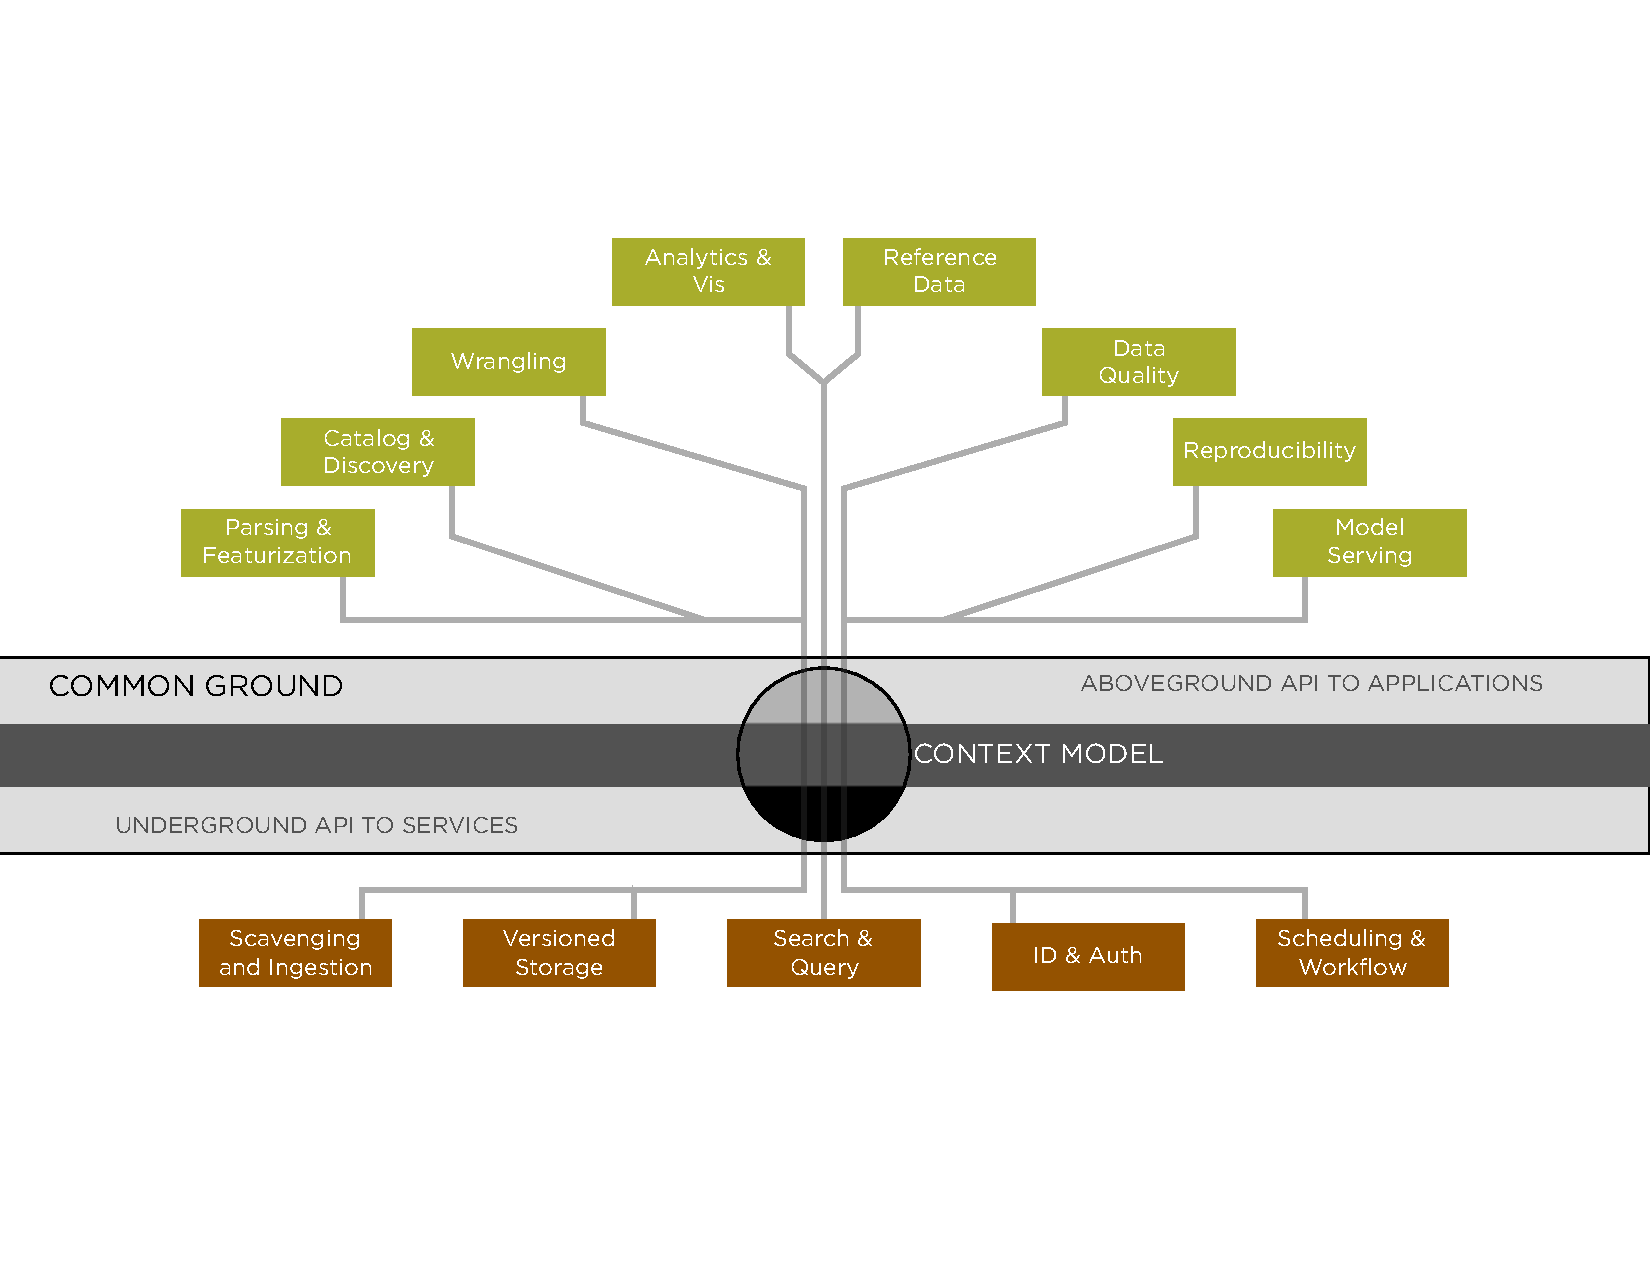
\includegraphics[width=0.75\linewidth]{groundarch.pdf}
\caption{The initial architecture of Ground.}
\label{fig:arch}
\end{figure*}
% \jmh{\textbf{Idea 3: A Pragmatic example in existing Hadoop workflows.  LinkedIn or Navigator customer story?}  Maybe take Idea 1 and make it less about assistive features, more about lost lineage across HDFS, Trifacta, Hive and Tableau?}

\section{Architecture of Ground}
\label{sec:arch}
Based on the requirements above, the Ground architecture is informed by Postel's Law of Robustness and the design pattern of decoupled components. 
At its heart is a foundational metamodel called \emph{Common Ground} with an associated \emph{Aboveground} API for data management applications like the catalog and wrangling examples above. 
The core functions underneath Ground are provided by swappable component services that plug in via the \emph{Underground} API. 
A sketch of the architecture of Ground is provided in Figure~\ref{fig:arch}.


\subsection{Key Services}
Ground's functionality is backed by five decoupled subservices.  For agility, we are starting the project using existing open source solutions for each.  We anticipate that some of these will require additional features for our purposes. In this section we discuss the role of each subservice, and highlight some of the research opportunities we foresee.  Our initial choices for subservices are described in Section~\ref{sec:prototype}.

\smallitem{Ingest: Insertion, Crawlers and Queues}.  Metadata may be pushed into Ground or require crawling; it may arrive interactively or in batches. 
% These kinds of services have been explored for data ingest, and only need modest modification for Data Context.  
The main issue is to decouple the systems plumbing of ingest from an extensible set of metadata and feature extractors.
To this end, ingest has both Underground and Aboveground APIs.
New context metadata arrives for ingestion into Ground via an Underground queue API. 
As metadata arrives, Ground publishes notifications via an Aboveground queue. Aboveground applications can subscribe to these events to add unique value, fetching the associated metadata and data, and generating enhanced metadata asynchronously. 
For example, an application can subscribe for file crawl events, hand off the files to an entity extraction system like OpenCalais or DeepDive, and subsequently tag the corresponding Common Ground metadata objects with  the extracted entities.
% Interactive insertion of metadata needs to be supported efficiently by the metadata storage component; batch insertion should make use of queueing services to handle bulk delivery and bursty arrivals.  
% Passive insertion needs to be handled via a data crawler that can register metadata from external services with Ground, and see if 
% We recently extended the LinkedIn Gobblin data ingest system to publish metadata for the objects it crawls (from 
% sources like filesystems, databases, etc.) into Ground via the Apache Kafka pub/sub system, which is made visible Aboveground. \vikram{Should we have this here or in our "State of the System" part? I think it makes more sense to keep them separate.}
% \joey{Attribute the systems to companies or cite them as apache projects.  Readers may not realize these are real widely used systems}
Metadata feature extraction is an active research area; we hope that commodity APIs for scalable data crawling and ingest will drive more adoption and innovation in this area. 
% Similarly, this is a rich area for industrial collaboration: the vendor-neutral aspect of Ground's plumbing should foster a healthy ecosystem of interoperable applications at higher levels.

\smallitem{Versioned Metadata Storage}.  Ground must be able to efficiently store and retrieve metadata with the full richness of the Common Ground metamodel, including flexible version management of code and data, general-purpose model graphs and lineage storage. 
% Ground also needs to reference external data and handle Schr\"{o}dinger versioning.  
While none of the existing open source DBMSs target this data model, one can implement it in a shim layer above many of them. 
We discuss this at greater length in Section~\ref{sec:perf}, where we examine a range of open-source DBMSs. As noted there, we believe this is an area for significant database research.

% Note that Ground is not intended as the primary interface for accessing the data that is referenced by metadata; Ground is expected to \emph{describe} external data and track it, not serve it.  Hence Ground's most basic requirement for external data is to know how to store a unique ID for each item it tracks, and return that ID to applications that request it.  In an ideal setting, each external data item is versioned, hence each version has a unique ID.  However if the external item is mutable and not versioned, Ground generates \emph{Schr\"{o}dinger versions} lazily: each time we observe an object we assume it changes, and assign it a new version (and version ID).  
% This is discussed in more detail in the Common Ground design~\cite{commonground}.

% \textbf{MVP:} We are currently mapping our metadata model onto a traditional PostgreSQL relational database for storage.  Graphs can be represented as relations, so we manage versions, lineage and data modeling graphs at application level above the relational model.  PostgreSQL is a fairly mature system but is not designed to meet our requirements for latency, scalability and availability. In fact we do not expect any relational solution to work well for our needs over time, as relational databases are not designed for any of the three key individual aspects of the metamodel: versioned data, polyglot data models, or rich lineage.  Unfortunately, we do not expect that solutions in the NoSQL or graph database world will fare well either, though this requires research to validate. Therefore a critical thrust of the Ground research agenda is to understand the weaknesses of existing database systems when faced with these requirements, and design a new database system that is well-suited to emerging metadata workloads. \jmh{Need to call out research hypotheses more clearly.}


\smallitem{Search and Analyze}.  Access to context information in Ground is expected to be complex and varied. As is noted later, Common Ground supports arbitrary tags, which leads to a requirement for search-style indexing.
%; we plan to integrate Solr~\cite{solr} and ElasticSearch~\cite{elasticsearch}.  
Second, intelligent applications like those in Section~\ref{sec:scenarios} will run significant analytical workloads over metadata---especially usage metadata which could be quite large.  
Third, the underlying graphs in the Common Ground model require support for basic graph queries like transitive closures. 
Finally, it seems natural that some workloads will need to combine these three classes of queries.
%, perhaps via a federated query layer above them.  
As we explore in Section~\ref{sec:perf}, various open-source solutions can address these workloads at some level, but there is significant opportunity for research here.

% \textbf{MVP:} Initially we are not supporting search or analytic APIs; these will be added as the system evolves.  For interactive query, we can only do as well as our prototype relational metadata store.  For search, we expect that existing solutions like Solr will be sufficient for the foreseeable future; we do not expect metadata tagging and querying to exceed volumes that Solr sees in free-text indexing. For analytics, we intend to leverage Spark and GraphX as we have significant expertise in house.  However, the nature of the analytics to be done here represents a major research opportunity: what might be the value of metadata in a Big Data context, and how could that value be extracted by analytics?  Could a \emph{self-aware} Big Data ecosystem improve itself, or provide valuable insight about its usage to applications and users?  \jmh{Again, call out research.}  Finally, the requirements for a federated query layer and its design are a topic for investigation after we acquire a corpus of metadata and workloads.

% \textbf{MVP:}  Currently we are handling ingest solely via simple push insertion APIs that call into our metadata store via SQL.  However we envision integrating open-source solutions like Kafka for queuing, and Gobblin for crawling and data ingest from remote sources.  We are also eager to explore APIs to plug in third-party solutions for  extracting metadata from crawled data; two examples we are OpenCalais (a free automated service for entity extraction) and Trifacta (a commercial, semi-automatic solution for data transformation).  We also recognize that there are boundless R\&D opportunities here, some of which could be part of Ground, many of which should exist as standalone solutions above Ground.  \jmh{another research opening, though more about opportunities above ground.}  We look forward to integration with other research and non-research colleagues here.

\smallitem{Identity and Authorization}.  
Identity management and authorization are required for a context service, and must accommodate typical packages like LDAP and Kerberos.  
Note that authorization needs vary widely: the policies of a scientific consortium will differ from a defense agency or a marketing department.  
Ground's flexible metamodel can support a variety of relevant metadata (ownership, content labels, etc.) 
% Ground's authorization APIs can be set synchronous to support enforcement policies, and/or asynchronous for post-hoc auditing.
% An open design question is whether Ground needs to \emph{enforce} policy, or merely store it and notify Aboveground applications.  
% \joey{I think we should emphatically not enforce the policy.  This would allow us to be more neutral and there is no way to in general enforce such a policy...  Perhaps we could instead provide tools for auditing ... }
Meanwhile, the role of versioning raises
subtle security questions.
Suppose the authorization policies of a past time are considered unsafe today---should reproducibility and debugging be disallowed? 
More research is needed integrate
versions and lineage 
with security techniques like Information Flow Control~\cite{zeldovich2008securing} in the context of evolving real-world pipelines.
% , and it's likely that most organizations would want to prevent version rollbacks in authentication policy. 
% More research is required here.

% \textbf{MVP:}  The current MVP has no support for identity management and authorization.  However our initial use case has us tracking UC Berkeley student IDs, Github identities, UNIX uids from instructional computing, and associations between the three; visibility of things like grading scripts and their outputs will depend on policies regarding these identities.  In the short term we expect to integrate with Google oAuth services as exposed at UC Berkeley next, and to explore the way that policy is specified and possibly enforced in our prototpype environment.  Our longterm roadmap here remains open; we expect a need to collaborate closely with partners in application domains to get further requirements.  \jmh{Possible tie to Raluca's work here, at minimum as an example of a non-standard approach to these issues.}

\smallitem{Scheduling, Workflow, Reproducibility}. 
We are committed to ensuring that Ground is flexible enough to capture the specification of workflows at many granularities of detail: from black-box containers to workflow graphs to source code.  
However, we do not expect Ground to be a universal provider of workflow execution or scheduling; instead we hope to integrate with a variety of schedulers and execution frameworks including on-premises and cloud-hosted approaches. 
This is currently under design, but the ability to work with multiple schedulers has become fairly common in the open source Big Data stack, so this may be a straightforward issue.

% \textbf{MVP:} We plan to begin by utilizing the scheduling and execution services provided by the Gobblin project, which supports a variety of schedulers including Quartz, Azkaban and Oozie, and execution frameworks including Yarn and Helix.  We plan to look into support for VMs and containers as well.  \jmh{Certainly could paint a research picture here, closer to the Bloom-meets-Kubernetes agenda: how will data-centric workflows be programmed in the future, especially as we look at containers, elastic services, etc?}  maybe also a connection to the Shenker/Jackson work on Declarative Datacenters?

\smallitembot
% \begin{figure*}[th]
% \center
% 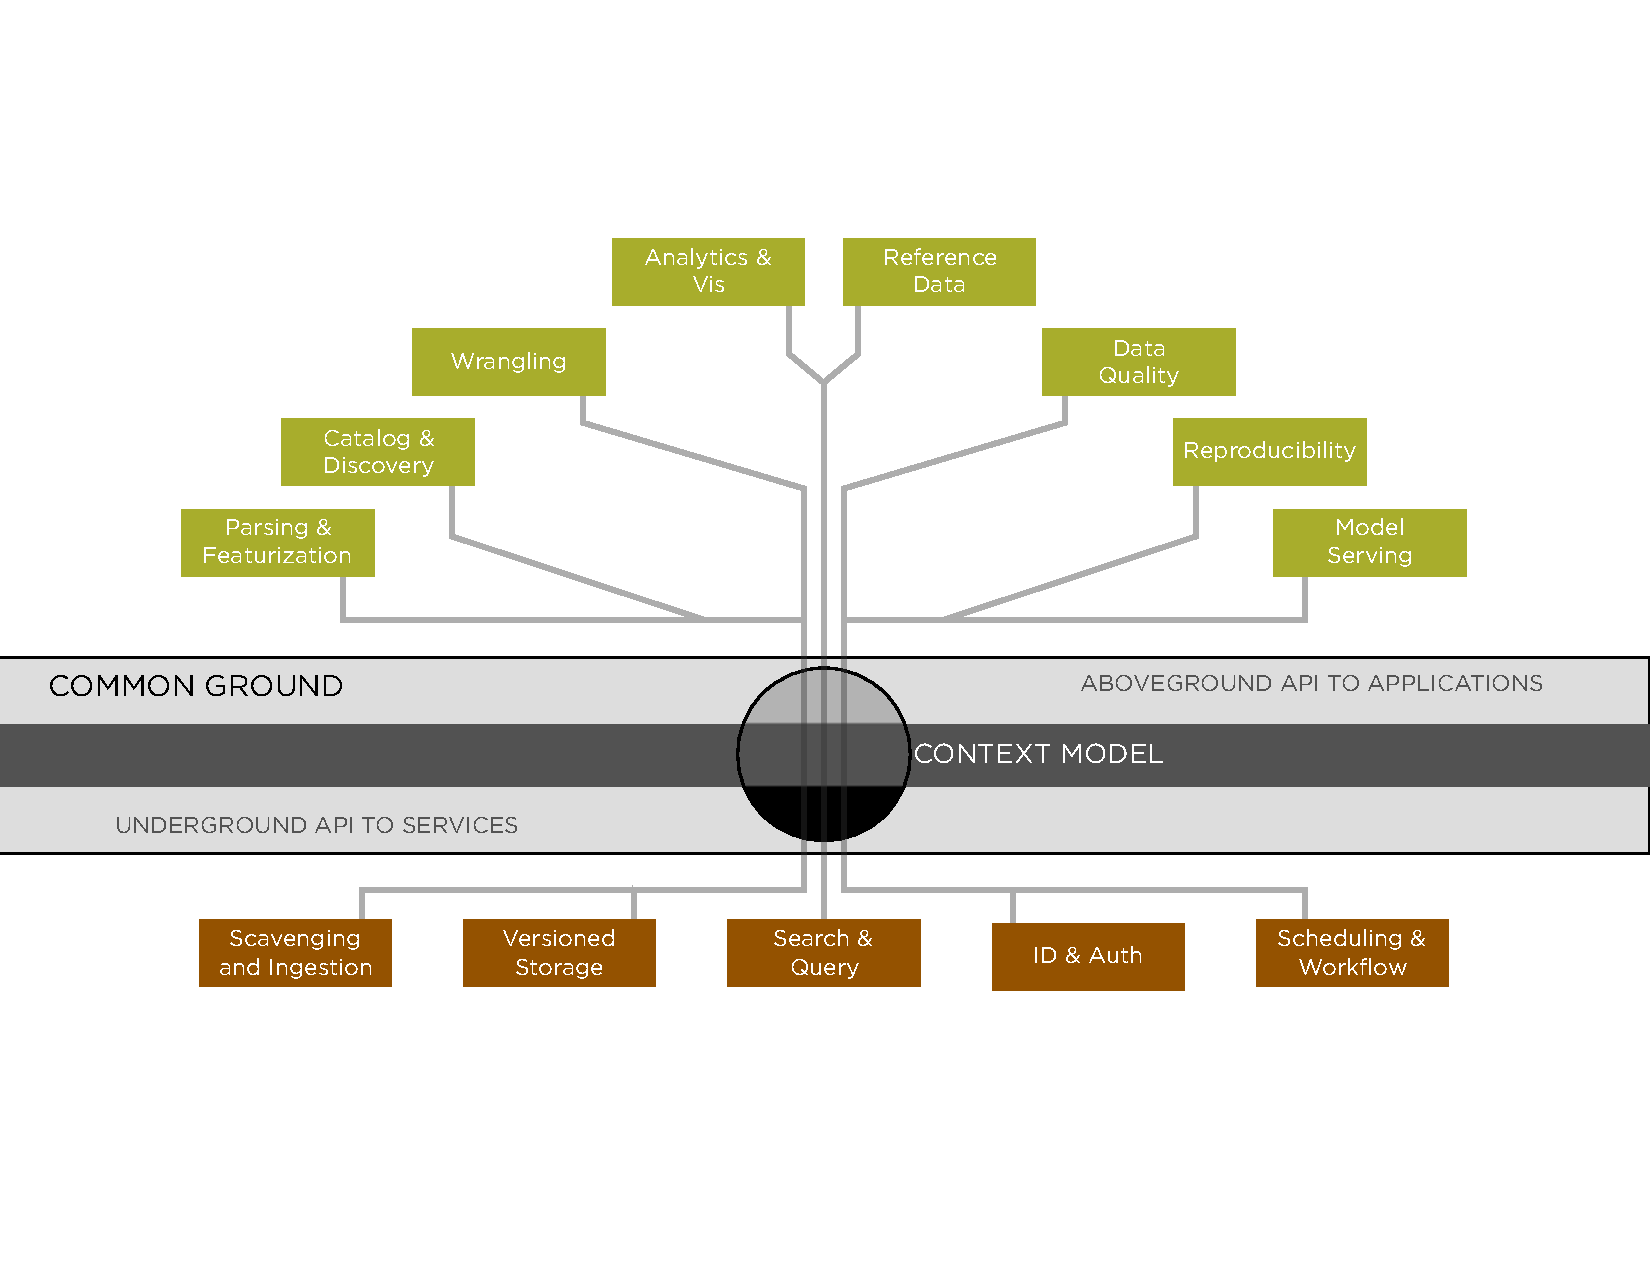
\includegraphics[width=0.7\linewidth]{groundarch.pdf}
% \end{figure*}

% \subsection{Common Ground: A Metamodel}
% \label{sec:metamodel}
% \subsection{Underground Services}


\begin{figure}[t]
\centering
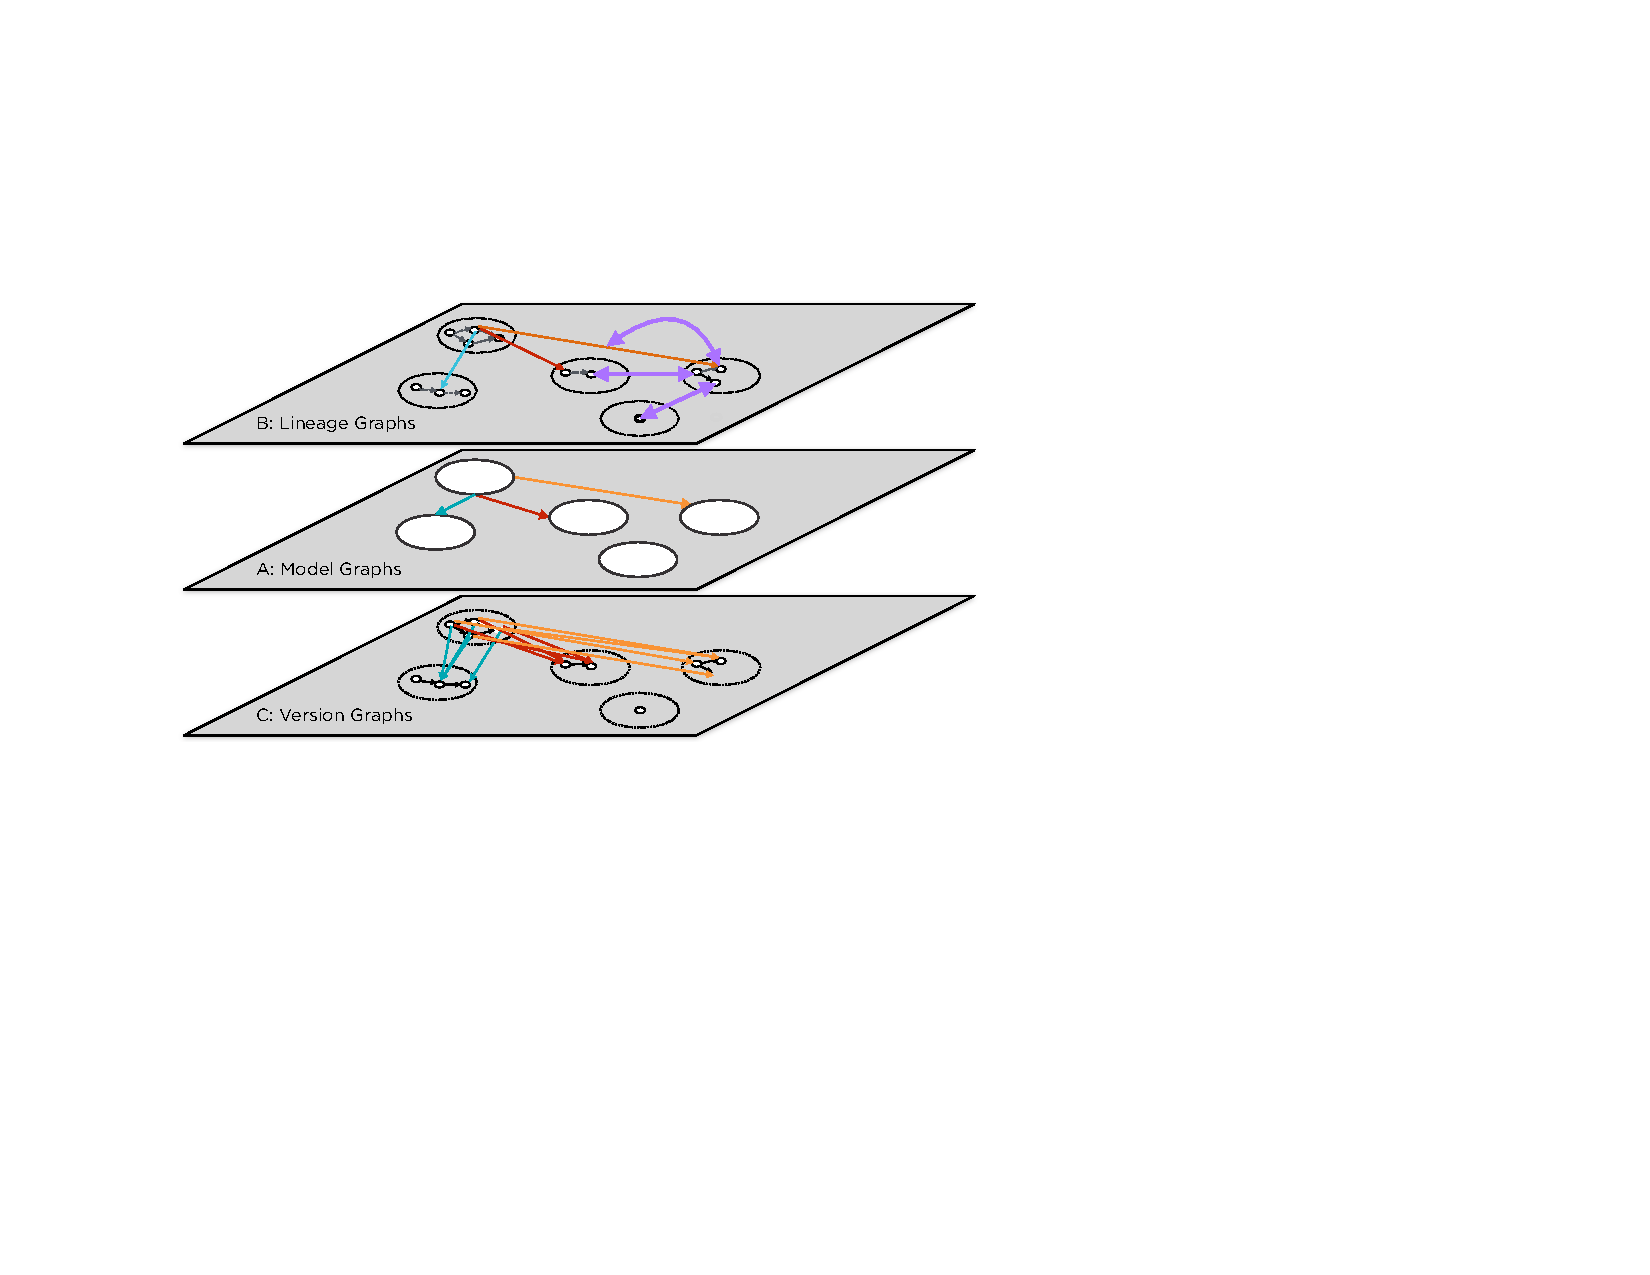
\includegraphics[width=\linewidth]{layers.pdf}
\caption{The Common Ground metamodel.} 
% The central layer shows {\node}s (circles) and {\edge}s.  
% Under are \kw{NodeVersion}s (small dots) corresponding to each \node, connected by \kw{EdgeVersion}s corresponding to each \edge.  
% Above is an example of lineage (dark edges) among selected versions.}
% For simplicity, the figure omits \kw{VersionSuccessor} relationships between different \kw{LineageEdgeVersion}s at the top, and between \
% \kw{EdgeVersion}s in the bottom layer.
\label{fig:layers}
\end{figure}

\subsection{The Common Ground Metamodel}
\label{sec:metamodel}
% \jmh{Pull in the practical motivation for each layer from the GDocs outline.}
Ground is designed to manage both the ABCs of data context and the design requirements of data context services.
The Common Ground metamodel is based on a layered graph structure shown in Figure~\ref{fig:layers}: one layer for each of the ABCs of data context.
% In the spirit of robustness, the central construct is simple and flexible: a Application-centric \modelgraph $M$ of nodes and edges for describing data, flexible enough to admit a diversity of traditional data models.
% (relational, entity/relationship, hierarchical, network, semi-structured, linked, etc.) 
% Underneath that metadata graph is a Change-capturing \versiongraph $V$, which can track a variety of models 
% of revision history for individual objects and collections. Above the metadata graph is a 
% Behavioral \lineagegraph $L$ used to capture the lineage of how pieces of data are derived.

%%%%%%%%%%%

\subsubsection{{\Core}s: Representing Change}
% \begin{figure}[ht]
% \begin{scriptsize}
% \begin{multicols}{2}
% % \lstinputlisting{scala/core.scala.txt}
% \end{multicols}
% \end{scriptsize}
% \caption{\Core metamodel in Scala.}
% \label{fig:core}
% \end{figure}
% \vikram{Rewrote this section and flipped the order of definitions to avoid redundancy.}

We begin with the \core layer of Common Ground, which the \emph{C} in the ABCs of data context. 
This layer bootstraps the representation of all information in Ground, by providing the classes upon which all other layers are based. These classes and their subclasses are the only information in Common Ground that is not itself versioned; this is why it forms the base of the metamodel.

The main atom of our metamodel is the \version, which is simply a globally unique identifier; it represents an immutable version of some object
depicted by the small circles in the bottom layer of Figure~\ref{fig:layers}. 
{\version}s can be linked into \kw{VersionHistoryDAG}s via \kw{VersionSuccessor} edges
indicating that one version is the descendant of another (the short dark edges in the bottom of Figure~\ref{fig:layers}.)
Type parametrization ensures that all of the \kw{VersionSuccessor}s in a given DAG link the same subclass of {\version}s together.
This representation of DAGs captures any partial order, and is general enough to reflect multiple different versioning systems.

To allow customization, the \core allows \version objects to be associated with
ad hoc {\gtag}s (key-value pairs) upon creation.
% {\version}s themselves are
% immutable, so this information has to be associated upon creation. 
Both {\version}s and {\gtag}s are themselves immutable.
% In more detail, we begin with the definition of a \thing, which is simply a unique ID and a \kw{VersionHistoryDAG}. 
% \kw{VersionHistoryDAG}s capture the change history across versions of a \thing; they consist of a set of \kw{VersionSuccessor}s that form a DAG of {\version}s representing branches and merges.


% The \core layer is not exposed to Aboveground (user-level) services. 
% Instead, it offers the base of an inheritance hierarchy that is exposed by the outer layers described Under.

%\kw{VersionHistoryDAG}s capture the change history across versions; they consist of a set of \kw{VersionSuccessor} relations that form a DAG of {\version}s representing branches and merges of versions. 
% Scala traits for the \core are shown in Figure~\ref{fig:core}.  
%(i.e., R transitively points to all other items). 
% Versioning forms the \core of Common Ground for two reasons.  
% First, we believe that context services are required to support complete history. 
% Metadata is long-lived, and key to understanding the evolving history of data---e.g., for auditing, reproducibility, and debugging. 
% Moreover, given the shrinking costs of storage and the increasing value of understanding data, metadata history is a good investment.
% % \footnote{Ground's design does not preclude the possiblity of truncating version history as a matter of system management, e.g., if storage is limited or policy dictates that certain metadata be retired.}.
% Second, 


% The last element of our \core metamodel is the critical building block for the rest of Common Ground: the \thing. 
%At the base of the hierarchy are identified, versioned objects called {\thing}s.
%A \thing consists simply of a unique ID and a \kw{VersionHistoryDAG}.
% \joey{You really need to give me more for Item, its still a little abstract of a concept ...}
% As we will see in the next section, most of the metamodel will use {\thing}s to capture the immutable aspects of an object, and the associated {\version}s to capture changes 
% to the object.

% \jmh{Do we want an equivalent of \tag for \thing?}
 
% \joey{This is also confusing.  How is the inheritance hierarchy exposed outsid }
% From this point on, when we speak of {\thing}s and {\version}s, we will actually be referring to objects in the subclasses defined Under that are visible above Ground.

\subsubsection{{\Mantle}s: Application Context}

% \begin{figure}[ht]
% \begin{scriptsize}
% \begin{multicols}{2}
% % \lstinputlisting{scala/mantle.scala.txt}
% \end{multicols}
% \end{scriptsize}
% \caption{\Mantle metamodel in Scala.}
% \label{fig:mantle}
% \end{figure}

% Our philosophy is that the metamodel should be designed in layers for
% simplicity and elegance. \core classes are shared and evolve in infrequent,
% regimented updates to maximize backwards compatibility. More detailed versions
% of the metamodel (including versions specific to use cases) are mapped onto
% simpler versions of the model. Our goal to find a balance between the
% simplicity and the expressivity of the metamodel and leave the rest up to the
% application using this metamodel.

% To illustrate this philosophy, we have developed a somewhat richer metamodel
% that can be imposed onto the aforementioned model.

The \mantle level of Common Ground provides a model-agnostic representation of application metadata: the \emph{A} of our ABCs. 
We use a graph model for flexibility: graphs can represent metadata entities and relationships from
semistructured (JSON, XML) and structured (Relational, OO, matrix) data models. A simple graph model enables 
the agility of schema-on-use at the metadata level, allowing diverse metadata to be independently captured as ad hoc model graphs and 
integrated as needed over time.

The \mantle is based on an internal superclass called \thing, which is simply a unique ID and a \kw{VersionHistoryDAG}. Note that 
an \thing is intrinsically immutable, but can capture change via its associated \kw{VersionHistoryDAG}: a fresh
\version of the \thing is created whenever a \gtag is changed. 

Ground's public API centers around three core object classes derived from \thing: {\node}, {\edge}, and {\graph}.
Each of these subclasses has an associated subclass in the \core: \kw{NodeVersion}, \kw{EdgeVersion} and \kw{GraphVersion}. {\node}s and 
{\edge}s are highlighted in the middle layer of Figure~\ref{fig:layers}, with the {\node}s projected visually onto 
their associated versions in the other layers.

The \core allows for ad hoc {\gtag}s, but many applications desire more structure.
To that end, the \mantle includes a subclass of \thing called {\structure}. A \structure is like a schema: a set of {\gtag}s that must be present. Unlike database schemas, the \structure class of Ground is versioned, via a \kw{StructureVersion} subclass in the \core.  If an \thing is associated with a \structure, each \version of the \thing is associated with a corresponding \kw{StructureVersion} and must define those {\gtag}s (along, optionally, with other ad hoc {\gtag}s.)
%If not, different {\version}s of the same \thing can optionally refer to different \kw{StructureVersion}s, recording evolution with regard to a choice of structures.  
Together, {\gtag}s, {\structure}s and \kw{StructureVersion}s enable a breadth of metadata representations: from unstructured to semi-structured to structured.

% Every \version of an \thing can optionally be associated with a \kw{StructureVersion}. If the associated \item 



% All of these objects and collections inherit from \thing, and hence are automatically versioned.   
% Scala traits for the Mantle are shown in Figure~\ref{fig:mantle}.
% typically with strong constraints on the graph shape (e.g. $\mbox{databases} \rightarrow \mbox{tables} \rightarrow \mbox{columns}$). %(Figure~\ref{fig:relational}).  
% \begin{figure}[ht]
% \centering
% \begin{minipage}{0.4\textwidth}
% 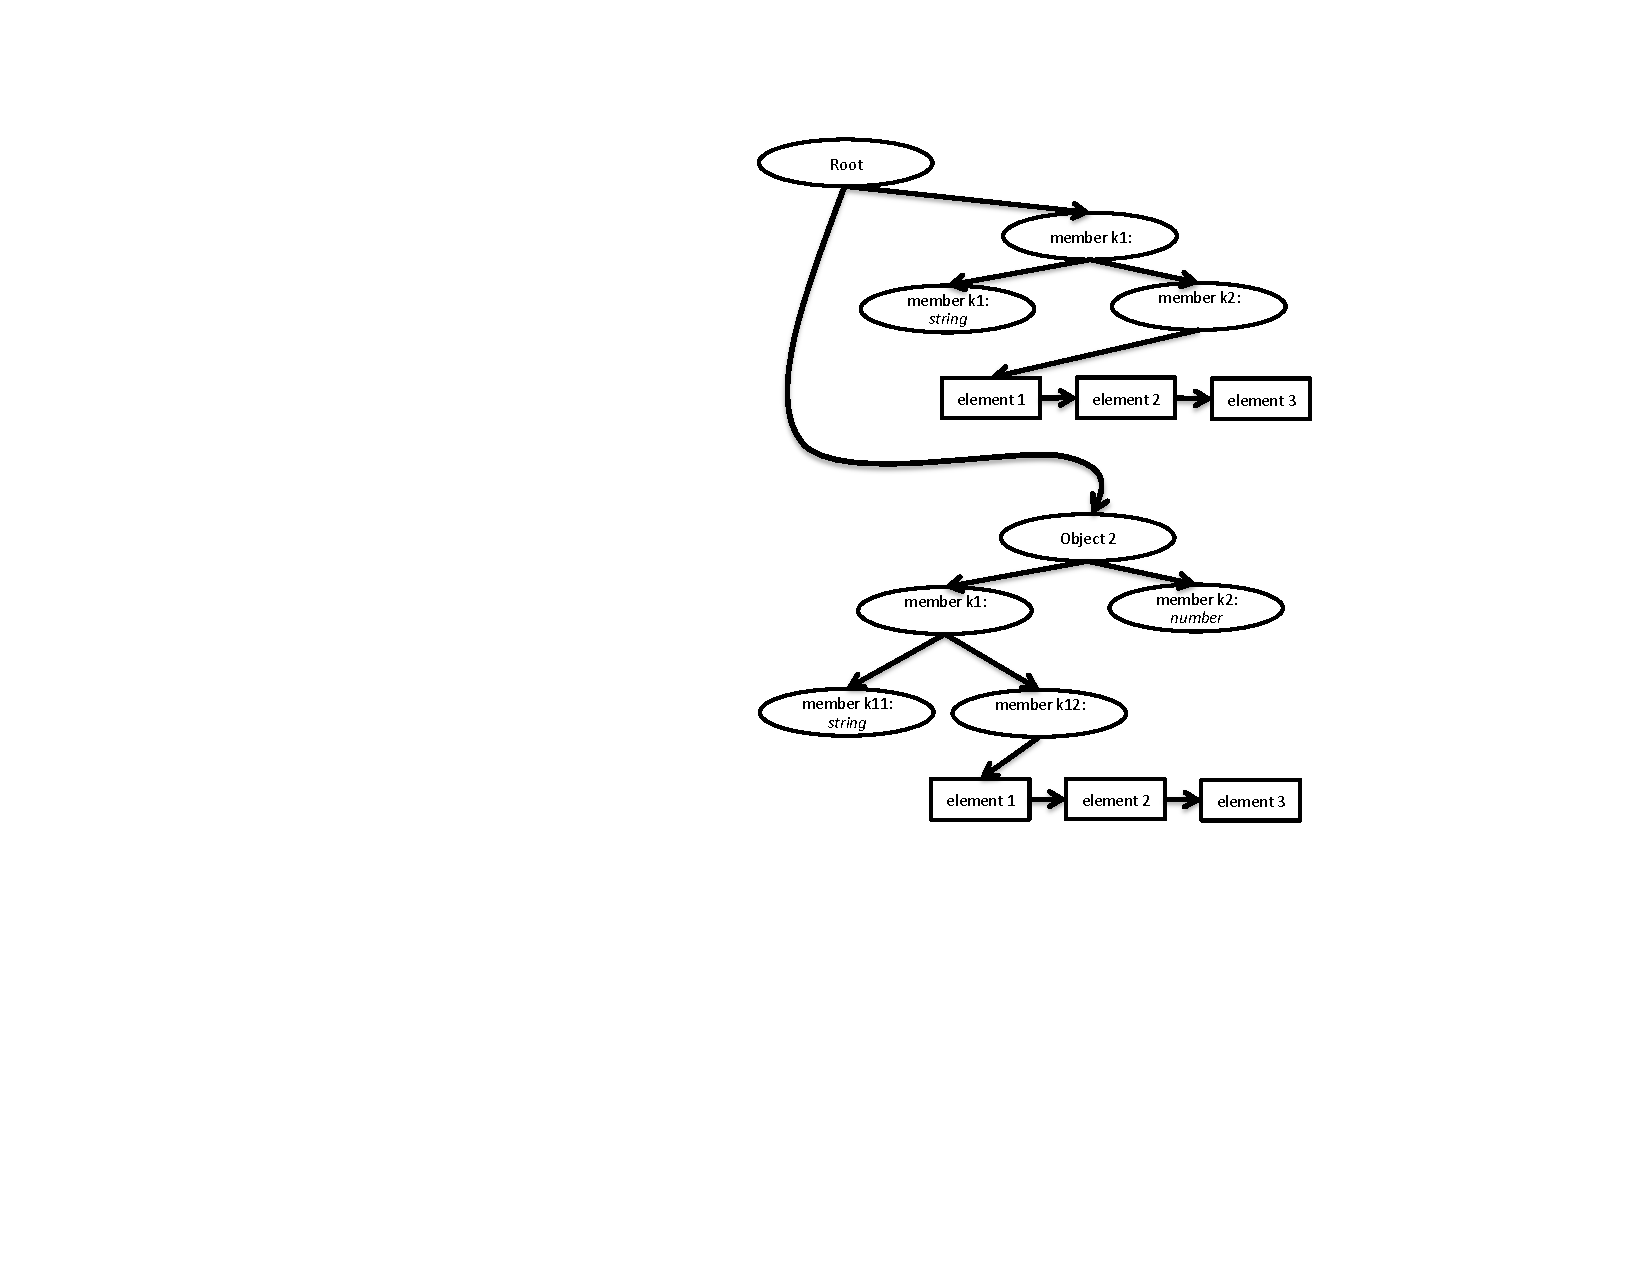
\includegraphics[height=2in]{json.pdf}
% \caption{A JSON document represented as a graph.  Note the nesting of JSON objects (key-value collections) in a tree shape of oval nodes, and lists as chains of rectangular nodes.}
% \label{fig:json}
% \end{minipage}
% \hspace{0.1\textwidth}
% \begin{minipage}{0.4\textwidth}
% 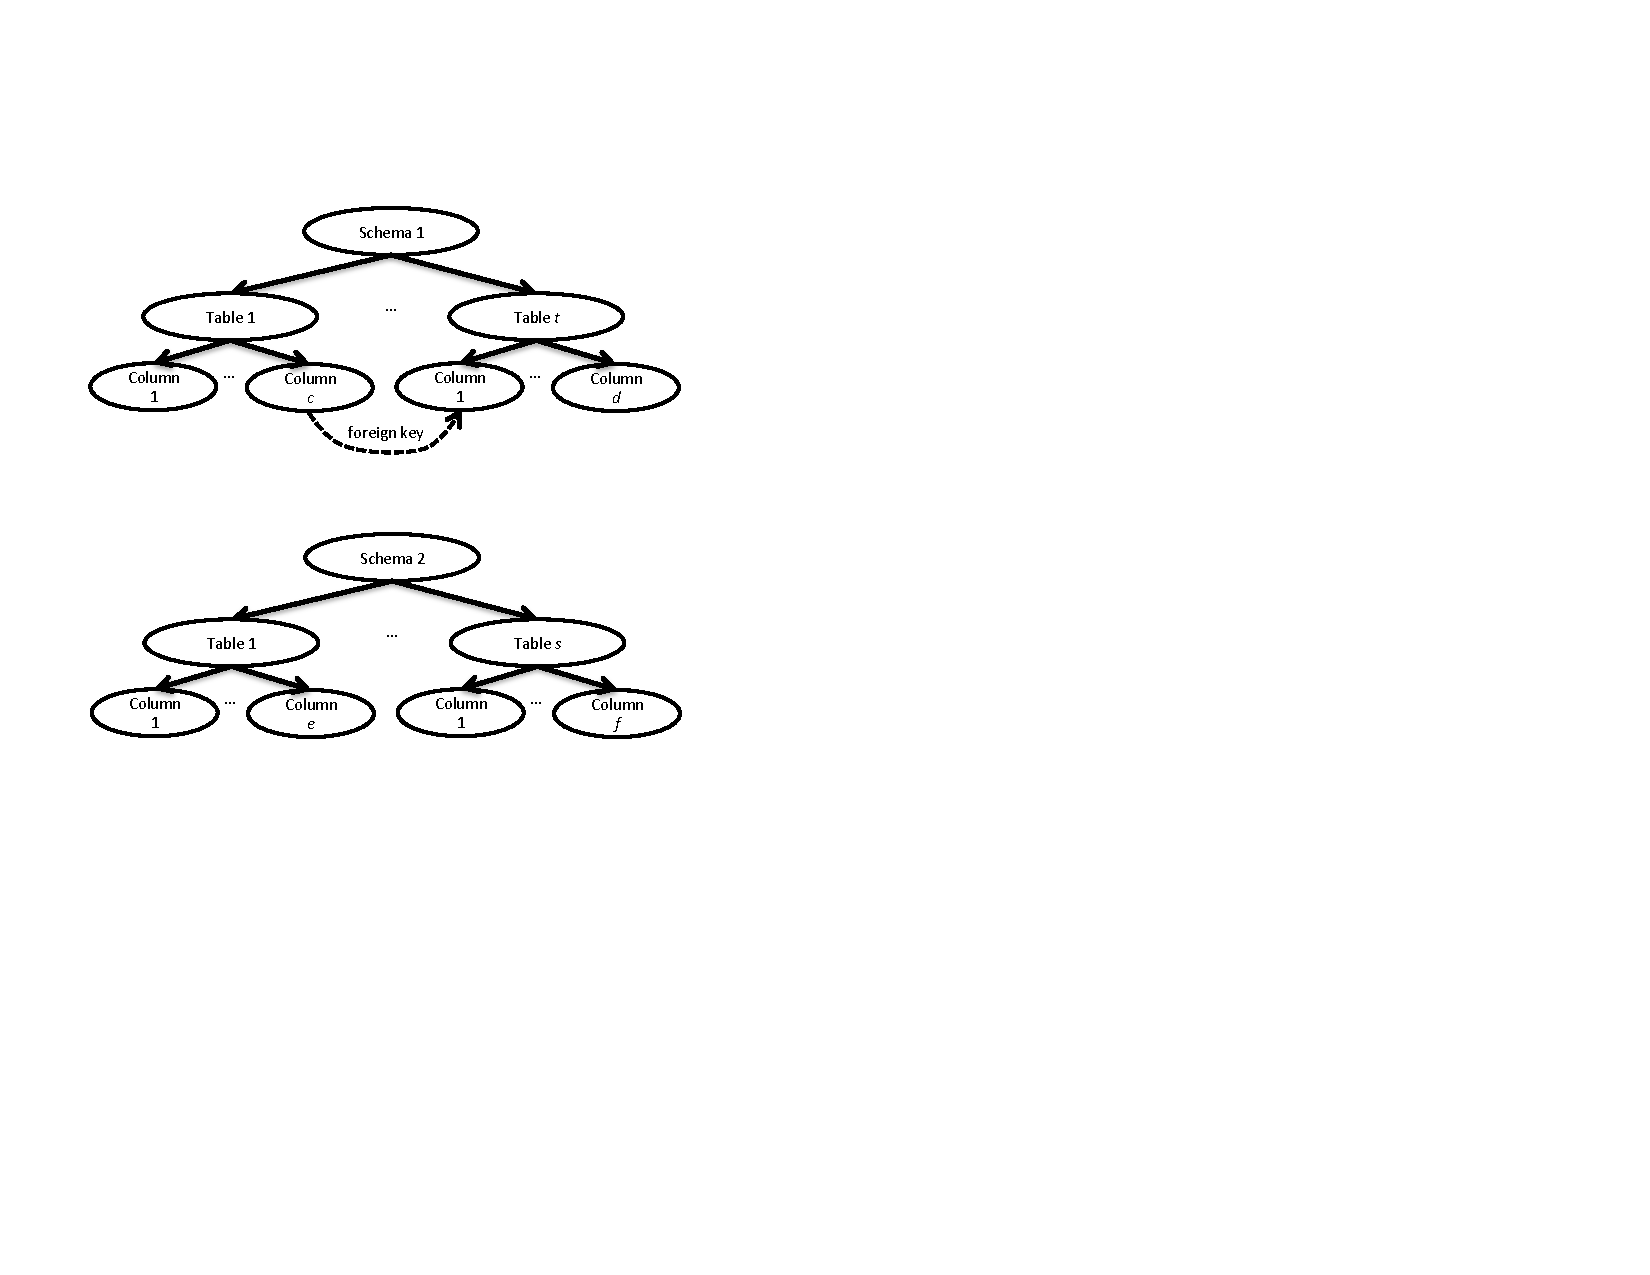
\includegraphics[height=2in]{relational.pdf}
% \caption{A relational database with two schemas, represented as a graph.  Note the fixed schemas$\rightarrow$tables$\rightarrow$columns structure, and
% the ad hoc foreign key references at the leaves.}
% \label{fig:relational}
% \end{minipage}
% \end{figure}

% The basic \mantle design consists of a user-extensible class hierarchy of matched pairs of \thing and \version subclasses: e.g., \node and \kw{NodeVersion}, \edge and \kw{EdgeVersion}, etc.
% These classes inherit from the \core model's \thing and \version classes respectively, imbuing a unique id as well as a \kw{VersionHistoryDAG} with each instance of $C$.  
% In turn, all {\version}s in a subclass like
% \kw{NodeVersion} are identified by a \kw{TVID} (Version ID) that stores
% both the ID of the corresponding \thing , and another \kw{VersionID}
% to distinguish the specific \version.  
% It is thus possible to determine {\thing}s
% from their {\version}s and vice versa.  
% \jmh{There is a 1-to-many constraint
% between {\thing}s and {\version}s.  Worth noting, and asserting somewhere in the
% code.} \vikram {We agreed that we didn't need actually add anything about this
% to the document, right?}
% \jmh{I skipped over RichVersions for simplicity.}
% \jmh{Careful here with tags -- associated with Items or Versions or both?}\vikram{Right now just Versions, but we've talked about adding them to Items as well.}
  % {\tag}s refer to the {\version} that contains them; 
  %a \tag is uniquely identified by its \version and key.  
% , a new \version subclass (e.g. \kw{NodeVersion}) must be generated to hold the new {\tag}s, and linked as a successor into
% the \kw{VersionHistoryDAG} of the corresponding \thing\footnote{Logically,
% the new version would likely contain a copy of all the unmodified {\tag}s
% of the preceding version as well, though in an implementation this could be
% encoded more efficiently.}.  
% We also allow {\tag}s to be associated with {\thing}s, 
% enabling users to register immutable tags that apply to all versions of a \thing.  \jmh{Need to get 
% this into the code.}  
% Structured information is captured via a \structure, akin to a relational table schema or a C struct. (This class is a descendant of \thing, hence contains versions in the form of \kw{StructureVersion}s.) {\structure}s provide a prescribed metadata format
% consisting of a set of key-type pairs; each \version that references a given \kw{StructureVersion} 
% \emph{must} have {\gtag}s with the corresponding 
% keys and value types.

% Up to this point we have referred to types rather loosely.  Ground currently includes 
% a typical set of built-in atomic types common to most languages: booleans, characters, strings, and
% numerics.  For now most of these types are being taken from Scala; we will evaluate whether additional 
% atomic types (e.g. SQL's decimal type) need to be built in.  One important type that is specific to 
% Ground is the Uniform Resource Identifier, or \uri.  We will describe the use of {\uri}s in more detail in the next section.  As of now we have no plans for user-defined types in Ground, though we will revisit
% this decision as we progress.
% As noted above, basic {\version}s are simply unique identifiers.
% We define {\richversion}s, which can be augmented with {\gtag}s and \kw{StructureVersion}s.  Our main user-facing modeling classes inherit from \richversion to support customization.  In general, the immutable aspects of \mantle model objects are captured in a \thing subclass
% (e.g. \node), and the mutable aspects in the corresponding \richversion subclass (e.g.
% \kw{NodeVersion}).  


% These basic objects are quite simple, but they can be customized by attaching
% ad hoc \kw{Attributes} to their versions: these are key/value pairs that can
% be attached to a specific \version. \jmh{Not clear from the Scala how you get attributes of a \thing!}
% Optionally, {\version}s can also have a \kw{Structure} that they impose: a set of attributes
% that they must contain.
% This more complex
% metamodel will simply be a composition of the building blocks we highlighted.
% The \mantle serves as the basis for increasingly rich, use-case specific forms of metadata that can be structured on top of this intermediate
% metamodel, benefiting both from the versioning embedded in the \core, and
% the typed graphical structure of the \mantle.
% The \node, \edge and \graph classes contain no more information than the \thing superclass provides; similarly the 
% \kw{NodeVersion} class contains no more than \version.
% %, albeit in a publicly visible interface.
% % However, both the
% % \kw{NodeVersion} and \kw{EdgeVersion} classes augment their \version
% % superclass with an optional reference to a \kw{StructureVersion} (that we
% % will describe shortly) to represent a required structure for the version.
% By contrast, \kw{EdgeVersion}s add two \kw{NodeVersion} endpoints; \kw{GraphVersion}s contain a set 
% of \kw{EdgeVersion}s.  
% Like other properties of a \version, that set is immutable.  Hence a new 
% \kw{GraphVersion} needs to be generated to capture the \graph being modified by insertion,
% deletion, or update of an existing \kw{EdgeVersion}.

  % Working through the definitions of
% Figure~\ref{mantle} you can see straightforward definitions of \kw{Set}s
% and \kw{SetVersion}s, which inherit from \thing and \version.  The \graph
% class inherits from \kw{Set} without modification; the
% \kw{GraphVersion} class extends \kw{SetVersion}.

  % \jmh{For symmetry, we should probably rename \version to Version, and \thing to something else like a Item.} \jmh{We need a naming convention for these things to avoid the goo of discussing objects and versions in an ad hoc way.}


% In the \mantle metamodel, we have a number of objects that each extend the
% \kw{VersionedItem}. For each of object (say) ``\kw{Foo}'', there is a
% corresponding ``\kw{FooVersion}''
% class.
% These classes extend the \version class and compose the \kw{VersionHistoryDAG}
% for the objects that they represent.

% We also have collections of {\node}s and {\edge}s. In order to illustrate the
% design of these collections, let's consider the example of a \graph, which is
% represented simply by a set of {\edge}s. A \graph, just like all the other objects
% in the \mantle, is a \thing. 
% Versions are more complex for a collection type like {\graph} than for scalar types like \node or \edge.
% A \graph's version can change in two different ways. The first is simple: when you add or delete an \edge from the \graph, you implicitly create a new
% version of the \graph container. The
% second is if the {\edge}s themselves are modified---in particular, when the
% endpoints of the \edge change, even though the identity of the edge may not\footnote{As a motivating example, consider an ``ownership'' \edge that represents the current owner of a file.  This fact does not change identity, it just links to a different principal as the owner, allowing us to track the ownership of that file over time.}. This second case poses an interesting challenge
% in terms of correctly propagating versioning changes. In order to solve this
% problem, every \thing has the capability of being ``watched''. That is,
% every object has a list of subscribers to which it publishes updates.
% In Ground, a \graph
% watches every one of its {\edge}s, and if an \edge is modified, then the \graph
% will also create a new version of itself with this \edge.  \jmh{This feels imperative.  Instead, how about a declarative description of a constraint: the version of a Graph relates in some way to the most recent version of any Edge it contains.  You could probably leave out the description of how this is achieved
% entirely.} \vikram{Maybe I'm not understanding what you mean by declarative
% here, but if you read up until the sentence that ends with "the identity of the
% edge may not, I think it describes the ways in which the identity of a graph
% depends on its edges. Beyond that, if we want to leave out a description of how
% we're accomplishing this, then we can just cut out everything after that,
% right? Or is there something else missing?}

\smallitem{External Items and Schr\"{o}dinger Versioning}\\
We often wish to track items whose metadata is managed outside of Ground: canonical examples
include GitHub repositories and Google Docs. Ground cannot automatically track these items as they change.
They are represented in Ground by \kw{ExternalItem}s, with \kw {ExternalVersion}s that contain various tags: a \kw{timestamp}, optional \kw{cachedValue}, and parameters for accessing the
reference (e.g., port, protocol, URI, etc.) 
% \vikram{We decided to remove these as standalone objects a while back. We instead just decided to have a concept of externality that was an add-on to existing objects. If what's here is the desired behavior, then I have some code to write. :-)}
% \jmh{I think it's OK to discuss if we believe it's a good idea..}
% \kw{ExternalItem}s have an \kw{isUnchanging}
% flag, which, if enabled, is an indication that the external resource is expected to be
% immutable, and there should only be one \kw{ExternalVersion} associated.
% Note that this is advisory; if the actual reference changes, Ground will not be aware. 
% Hence
% (i.e., not \kw{isUnchanging}), 
Whenever a Ground client uses the Aboveground API to access an a \kw{ExternalVersion}, this results in Ground fetching the object and generating a new \kw{ExternalVersion}, containing a new
\kw{VersionID}, an updated timestamp and possibly an updated cached value. We refer to this as a \emph{Schr\"{o}dinger} versioning scheme: each time we observe an \kw{ExternalItem} it changes. This allows Ground to track the history of an external object \emph{as perceived} by Ground-enabled applications.

% In summary, the \mantle model provides a public, above-Ground interface for building application-specific 
% abstractions by customizing the optional and structured tags of nodes and edges, and laying them out in versioned graphs. 

\subsubsection{{\Crust}s: Behavior}
% \begin{figure}[ht]
% \begin{scriptsize}
% \begin{multicols}{2}
% % \lstinputlisting{scala/crust.scala.txt}
% \end{multicols}
% \end{scriptsize}
% \caption{\Crust metamodel in Scala.}
% \label{fig:crust}
% \end{figure}
The goal of the \crust layer is to capture usage information composed from the nodes and edges in the model graph.  
To facilitate data lineage, Common Ground depends on two specific items---
principals and workflows---that we describe here.
% These are the only two items in Common Ground that go beyond graph structure; they are fundamental to the semantic notion of lineage.

\kw{Principal}s (a subclass of \node) represent the actors that work with data:  users, groups, roles, etc. 
% \kw{Principal}s are particularly important in data governance
% because they are central to both auditing and
% enforcement of policies like access control.
% Note that \kw{Principal}s
% are {\node}s, and built while access rights and group membership can be represented as {\edge}s.
% {\structure}s would be particularly useful here because users would
% have some set of required information based on the identity \& authentication
% schemes being used. 
\kw{Workflow}s (a subclass of {\graph}) represent specifications of code that can be invoked. Both of these classes have associated \kw{Version} subclasses.
% \kw{Principal}s and \kw{Workflow}s
% are the only ``semantic'' metadata objects prescribed by Common Ground; the rest of the metamodel is 
%  structural and general-purpose.
Any Data Governance effort requires these classes: as examples, they are key to
authorization, auditing and reproducibility.

% The second common semantic concept is \emph{workflow specification}.
% This sort of metadata is very important to critical use cases like reproducibility and auditing.
% Workflows are representable in terms of the graph
% structure of the \mantle model, but we chose to make them
% first-class citizens in the \crust of the Ground metamodel. These
% This is critical to use cases like reproducibility and auditing.

% \kw{Workflow}s
% can capture a sequence of \textit{ad hoc}, exploratory actions or a
% pre-defined sequence of actions. 

In Ground, lineage
is captured as a relationship between two {\version}s. 
This relationship is due to some process, either computational
(a workflow) or manual (via some principal). \kw{LineageEdgeVersion}s (purple arrows in the top layer of Figure~\ref{fig:layers}) connect two or more (possibly differently-typed) {\version}s, at least one of which is a \kw{Workflow} or \kw{Principal} node. 
Note that \kw{LineageEdgeVersion} is not a subclass of \kw{EdgeVersion}; an \kw{EdgeVersion} can only connect two \kw{NodeVersion}s; a \kw{LineageEdge} can connect {\version}s from two different subclasses, including subclasses that are not under \kw{NodeVersion}.  
For example, we might want to record that Sue imported \kw{nltk.py} in her \kw{churn.py} script; this is captured by a \kw{LineageEdge} between a \kw{PrincipalVersion} (representing Sue) and an \kw{EdgeVersion} (representing the dependency between the two files).  

% \jmh{This paragraph can be chopped for space.}
% Usage data is often generated by analyzing log files, code, and/or data, and it can become very large.
% There are important choices about how and when to materialize lineage that are best left to applications. For example, in a pure SQL environment, the lineage of a specific tuple in a table might be materialized on demand as a tree of input tuples, but the lineage for all tuples in the table is more efficiently described by version IDs for the SQL query and its input tables. Ground can support both, but 
% does not dictate a choice.
% % To support such lazy evaluation, \emph{ephemeral} \kw{LineageEdgeVersion}s can be generated in the Ground lineage API without materializing the (redundantly computed) \kw{LineageEdgeVersion}s in immutable storage. 
% % \vikram{I'm confused about what this is saying. 
% % It definitely doesn't exist in the code. :-)}

\subsubsection{Extension Libraries}
The three layers of the Ground metamodel are deliberately general-purpose and non-prescriptive.
We expect Aboveground clients to define custom \kw{Structure}s to capture reusable application semantics.  
These can be packaged under {\node}s representing shared libraries---e.g., a library for representing
relational database catalogs, or scientific collaborations. \kw{StructureVersion}s allow these to be evolved over time in an identifiable manner.

% The API for \groundwire is the subject of a separate document.

%%%%%%%%%%%


\section{Ground \lowercase{v}0}
\label{sec:prototype}

% \subsection{State of the System}
Our initial version of Ground implements the Common Ground metamodel and provides REST APIs for interaction with the system. 
It currently makes use of LinkedIn Gobblin for crawling and ingest and Apache Kafka for queueing and pub/sub.
We have integrated and evaluated a number of backing stores for versioned storage, including PostgreSQL, Cassandra, TitanDB and Neo4j; we report on results later in this section.
% An integral part of our initial architecture has been evaluating different "state of play" backing stores. 
% In particular, Ground currently is compatible with Postgres, Apache Cassandra, TitanDB, and Neo4j. 
We are currently integrating ElasticSearch for text indexing and are still evaluating options for Authorization and Scheduling. 


% % This pipeline notifies us of any new files that are added to HDFS. 
% % In addition, we are planning on adding hooks which allow Ground to call out to other services (e.g., a parser or featurizer that will extract additional metadata) that might be interested in new files. 

% \smallitem{Code Versions: Git History.} Another key kind of metadata is code versions; as described in the introduction, code it key to understanding the meaning and usage of data.
% Today, a great deal of code is versioned in git repositories.
% % An integral part of tracking data usage effectively is understanding which code versions were used to transform or wrangle data. 
% To that end, we have ingested version history graphs from git repositories into Ground.
% \smallitembot


% % These three use cases represent three very different kinds of metadata, exercising the flexibility of our model graphs and underlying storage. Git has a fairly rich versioning model, which exercises our version graphs. Together these use cases


To exercise our initial design and provide immediate functionality,
% ``out of the box'', 
we built
% provide 
support for three sources of metadata most commonly used in the Big Data ecosystem: file metadata from HDFS, schemas from Hive, and code versioning from Git.
To support HDFS, we extended Gobblin to extract file system metadata from its HDFS crawls and publish them to Ground's Kafka connector. The resulting metadata is then ingested into Ground, and notifications are published on a Kafka channel for applications to respond to. To support Hive, we built an API shim that allows Ground to serve as a drop-in replacement for the Hive Metastore.
One key benefit of using Ground as Hive's relational catalog is Ground's built-in support for versioning, which---combined with the append-only nature of HDFS---makes it possible to \emph{time travel} and view Hive tables as they appeared in the past.  To support Git, we have built crawlers to extract Git history graphs as \kw{ExternalVersion}s in Ground. These three scenarios guided our design for Common Ground.

Having initial validation of our metamodel on a breadth of scenarios, our next concern has been the efficiency of storing and querying information represented in the Common Ground metamodel, given both its general-purpose \mantle layer, and its support for versioning. To get an initial feeling for these issues, we began with two canonical use cases:

\smallitem{Proactive Impact Analysis.} A common concern in managing operational data pipelines is to assess the effects of a code or schema change on downstream services.
As a real-world model for this use case, we took the source code of Apache Hadoop and constructed a dependency graph of file imports that we register in Ground.
We perform impact analysis by running transitive closure starting from 5,000 randomly chosen files, and measuring the average time to retrieve the transitively dependent file versions.

\smallitem{Dwell Time Analysis.} In the vein of the analysis pipeline Sue manages in Section~\ref{sec:scenarios}, our second use case involves an assessment of code versions on customer behavior. 
In this case, we study how user ``dwell time'' on a web page correlates with the version of the software that populates the page (e.g., personalized news stories). 
We used a sizable real-world web log ({\small \url{http://waxy.org/2008/05/star_wars_kid_the_data_dump/}}) %~\cite{starwarskid}, 
but had to simulate code versions for a content-selection pipeline. 
To that end we wanted to use real version history from git; in the absence of content-selection code we used the Apache httpd web server repository. 
Our experiment breaks the web log into sessions and artificially maps each session to a version of the software.
We run 5,000 random queries choosing a software version and looking up all of its associated sessions.
\smallitembot

While these use cases are less than realistic both in scale and in actual functionality, we felt they would provide simple feasibility results for more complex use cases.

\subsection{Initial Experiences}
\label{sec:perf}
To evaluate the state of off-the-shelf open source, we chose leading examples of relational, NoSQL, and graph databases.
All benchmarks were run on a single Amazon EC2 \kw{m4.xlarge} machine with 4 CPUs and 16GB of RAM. 
Our initial goal here was more experiential than quantitative---we wanted to see if we could easily get these systems to perform adequately for our use cases and if not, to call more attention to the needs of a system like Ground.
We acknowledge that with further tuning, these systems might perform better than they did in our experiments, though we feel these experiments are rather fundamental and should not require intensive tuning.

\begin{figure}
\centering
\begin{minipage}{.5\linewidth}
  \centering
  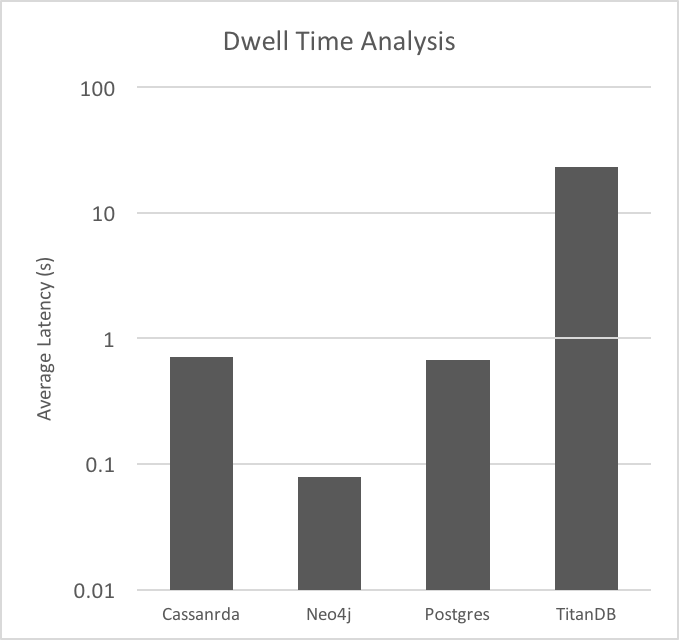
\includegraphics[width=\linewidth]{adjacent.png}
  \caption{Dwell time analysis.}
  \label{fig:dwell}
\end{minipage}%
\begin{minipage}{.5\linewidth}
  \centering
  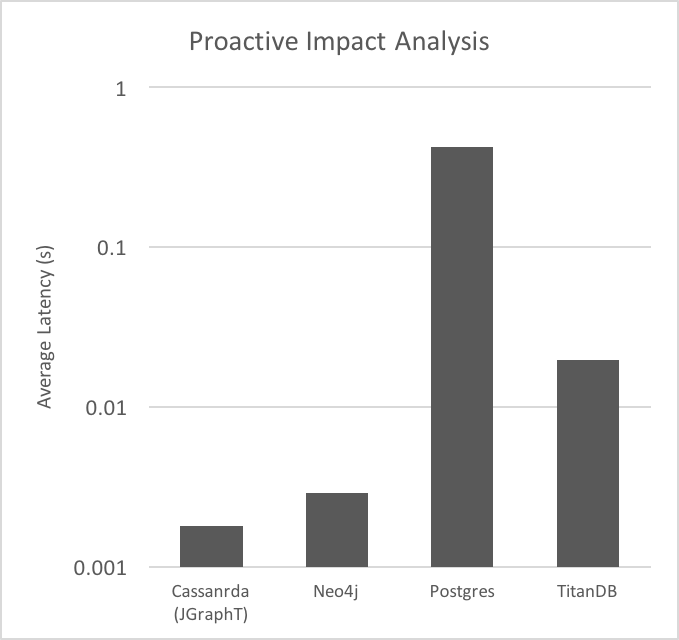
\includegraphics[width=\linewidth]{trans_closure.png}
  \caption{Impact analysis.}
  \label{fig:impact}
  \end{minipage}
 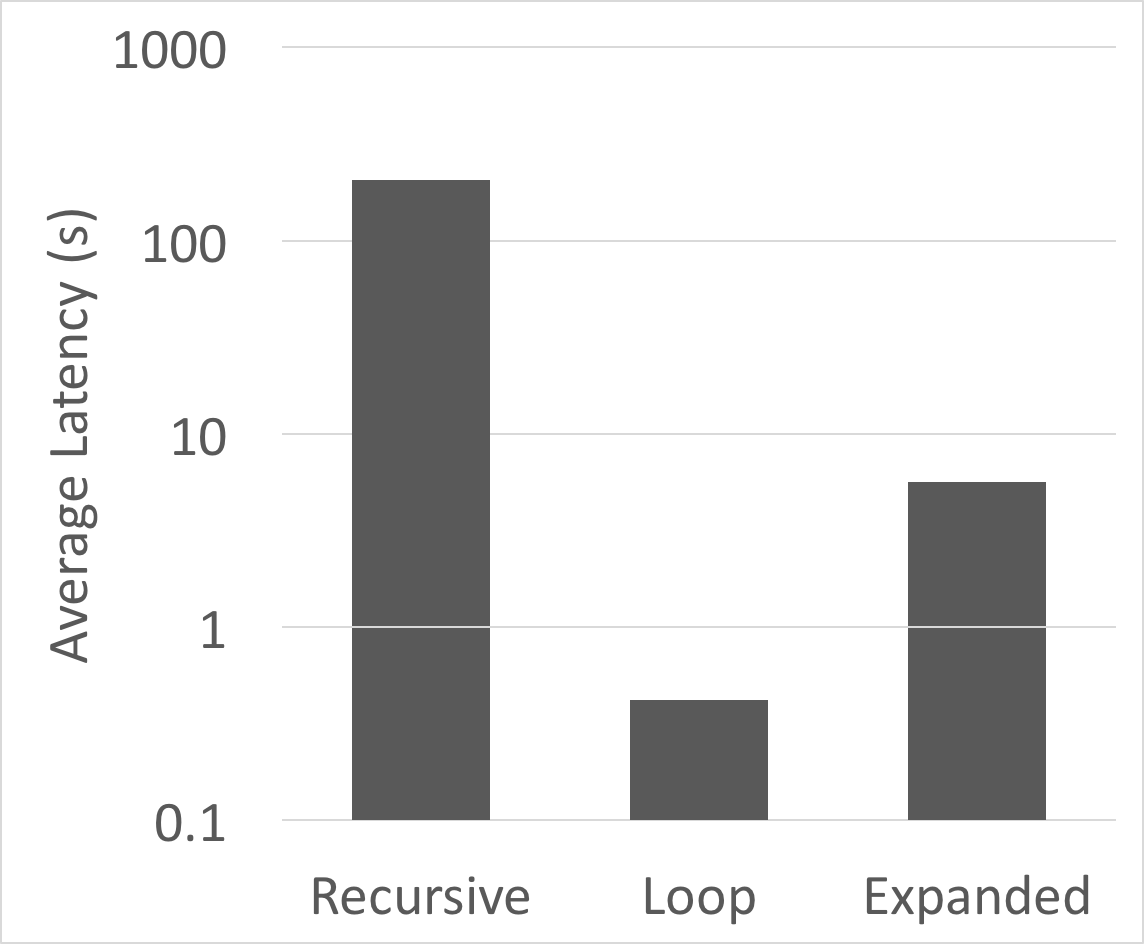
\includegraphics[width=0.5\linewidth]{postgres.png}
  \caption{PostgreSQL transitive closure variants.}
  \label{fig:postgres}
\end{figure}


\smallitem{PostgreSQL}. We normalize the Common Ground entities 
(\thing, \version, etc.) into tables, and the relationships
(e.g., \kw{EdgeVersion}) into tables with indexes on both sides. 
The dwell time analysis amounts to retrieving all the sessions corresponding to a server version; it is simply a single-table look-up through an index. The result set was on the order of 100s of nodes per look-up.
% The performance results here are expected and not noteworthy.

For the impact analysis experiment, we compared three PostgreSQL implementations. The first was a \kw{WITH RECURSIVE} query. 
The second was a UDF written in PGPLSQL that computed the paths in a (semi-naïve) loop of increasing length. 
The last was a fully-expanded 6-way self-join that computed the paths of the longest possible length. Figure~\ref{fig:postgres} compares the three results; surprisingly, the UDF loop was faster than the native SQL solutions. 
Figure~\ref{fig:impact} shows that we were unable to get PostgreSQL to be within an order of magnitude of the graph processing systems. 
% with even the fastest implementation.

\smallitem{Cassandra}. In Cassandra, every entity and relationship from the Common Ground model is represented as a key/value pair, indexed by key. 
The Cassandra dwell time analysis query was identical to the Postgres query: a single table look-up which was aided by an index.
% Cassandra can be integrated with an in-memory Java graph-processing library called JGraphT to answer the query. 
Cassandra doesn't support recursive queries; for impact analysis, we wrapped Cassandra with JGraphT, an in-memory Java graph-processing library. We did not count the time taken to load the graph into JGraphT from Cassandra, hence Figure~\ref{fig:impact} shows a very optimistic view of Cassandra's performance for this query.

\smallitem{Neo4j}. Neo4j is a (single-node) graph database, so modeling the Common Ground graphs was straightforward.
The average Neo4j dwell time analysis was fast; the first few queries were markedly slow
(${\sim}10$ seconds),
but subsequent queries were far faster, presumably due to caching. 
% \jmh{We should discuss hot vs. cold performance in the experimental setup. Any effects for other systems?}
Neo4j excelled on transitive closure, performing only 50\% slower than in-memory JGraphT.
% With both queries, performance was significantly bolstered by indexing the \kw{NodeVersion} id that served as the starting point.

\smallitem{TitanDB}. TitanDB is a scale-out graph database designed to run over a NoSQL database like Cassandra, which is how we deployed it in our experiments on a single machine. % \jmh{right?} 
Once again, mapping our graph-based model into TitanDB was straightforward.
TitanDB's dwell time analysis performance was significantly slower than the rest of the systems, despite indexing.
The impact analysis query was significantly faster than any Postgres implementation but was still an order of magnitude slower than Neo4j and JGraphT. 

\smallitembot
While there is variance in our simple dwell time analysis lookups, the bigger divergence is in the impact analysis workload.
We can expect impact analysis to traverse a small subgraph within a massive job history. Queries on small subgraphs should be very fast---ideally as fast as an in-memory graph system~\cite{mcsherry2015scalability}. JGraphT-over-Cassandra and Neo4j provide a baseline, though neither solution scales beyond one node. PostgreSQL and TitanDB do not appear to be viable even for these modest queries. Of these systems, only Cassandra and TitanDB are designed to scale beyond a single node.

% \section{Discussion}
% \label{sec:discussion}
% \jmh{This may evolve into Research Opportunities or Future Work, but this is a placeholder for things that were postponed in earlier text}

% \jmh{Backref to Scalability discussion above, and the question ``are logs data or metadata''?}
% Functionality: well, we've started building out a few things and they went well.  Apiary and Grit.

% Performance: Here we ran into some bottlenecks with the widely-used storage systems in the field.  This merits more attention.

% \section{Challenges for the community}
% \label{sec:challenges}
% \jmh{May not be room for this. Instead find a way to call out the challenges in the body as they occur, with clear formatting.}

\section{Related Work}
\label{sec:relwork}
% \joey{made a pass on this section and it looks good}
Work related to this paper comes in a variety of categories. 
For submission brevity, we focus on related system architectures and omit bibliography entries to systems easily found online. 
An accepted version will contain a more scholarly bibliography.


% Legacy 
Classic commercial Master Data Management and ETL solutions were not designed for 
schema-on-use or agility. 
Still, they influenced our thinking and many of their features should be supportable as a subset of the Ground functionality~\cite{loshin2010master}.
% While this is unnatural in today's agile environments, it is interesting to consider what can be salvaged. 
% % Can curation invariants be inferred rather than authored? 
% % If they are ``soft'' invariants, how should software and organizations maintain them? 
% % What kinds of user experiences can blend the governance of traditional tools with the agility of ad hoc analytics?  
% % This is an excellent opportunity for innovation. 
% Meanwhile, readers familiar with these systems will be able to map them into parts of our ABCs of context: ``business'' metadata falls into Category A, while ``technical'' or ``operational'' metadata'' falls into both A (for system specs) and B (for usage and lineage).
Meanwhile,
two emerging metadata systems address governance for Big Data: Cloudera Navigator and the Hortonworks-led Apache Atlas. 
Both provide graph models that inspired the Common Ground \mantle; neither provides versioning or is perceived as vendor-neutral. % These systems are also exploring ``underground'' alternatives for storage.

There is a broad space of efforts that illustrate the possibilities of data context. 
There are many applications and research projects for tasks like cataloging, wrangling, and lineage analysis. 
OpenChorus and IBM LabBook provide portal-type applications for collaboration and social data analysis.
LinkedIn WhereHows, FINRA Herd and Google Goods are metadata services built to support data workflows in their respective organizations; Goods bundles what we call Underground services with various proprietary services we might describe as Aboveground applications.
% Alation, Tamr, Waterline,
% ReproZip, Burrito
% DeepDive, OpenCalais
% VizTrails
All of the above make use of specific metamodels customized to their needs. By contrast, Ground is focused on designing a reusable service to enable diverse applications and organizations to integrate their notions 
of data context. 
This changes the challenges and opportunities we are pursuing, and hopefully will encourage broader adoption and innovation.


% Custom metadata stores have been open-sourced by LinkedIn (WhereHows) and FINRA (Herd); both of these are ``opinionated'' rather than general-purpose: specific to use cases in their organizations. They provide a good challenge for Ground, as examples of use cases to be supported. 

% As noted in Section~\ref{sec:scenarios} 
% There are also many Aboveground commercial and research tools for extracting features and lineage, and providing visual interfaces to those kinds of metadata.
% Today, these systems must track their own context and metadata, and have to implement point-to-point integrations with other applications and services. 
% Our hope is that Ground will accelerate this activity and enable these applications to improve substantially in coming years.


% Postgres, DataHub, Datomic Pachyderm, Noms
Our initial assessment of storage engines suggests a need for more work: both a deeper evaluation of what exists and very likely designs for something new. There are many research papers and active workshops on graph databases (e.g., \cite{grades16}), but we found the leading systems (Neo4j, Titan) lacking. 
% \joey{should we breifly say how?}\jmh{Implicit in perf section. space is very short.} \joey{fair}
Interest in no-overwrite databases has only recently reemerged, including the DataHub research project, and the Datomic, Pachyderm and Noms systems.  The combination of these two kinds of functionality 
appears to be a new challenge.
% In future work we plan to assess this space more deeply. \joey{not sure what we mean by assess this space?  Perhaps we want to say: In the future we plan to revisit many ideas (e.g., ) in these earlier systems as we develop systems for metadata management.}\joey{addressed!}

% including Big Data catalog applications (Alation, Tamr, Waterline), analytic lineage systems (ReproZip, Burrito), information extraction systems (DeepDive, OpenCalais, etc.) and so on. Our hope is for Ground to provide a widely adopted, interoperable subsystem for these applications, freeing them to focus on their own key technical differentiators in adding application-specific intelligence and user experiences.  Finally, there is a host of research on graph queries/DBs, and a much smaller body of work on immutable databases (Postgres, Datomic, Pachyderm.io, Noms); it is quite possible that those solutions could evolve to serve the needs of a context service like Ground.  \textbf{Mention VizTrails.}

% Readers familiar with 20th Century enterprise metadata products should recognize how terminology of that era fits into this broadened scope. ``Business metadata'' like compliance details, keywords, and classifications fall into Application context. Some ``technical metadata''  (configurations and scripts) fit into Application context; data lineage by contrast fits into Behavioral Context. ``Operational metadata'' regarding execution fits into Behavioral Context as well.

\section{Conclusion}
\label{sec:conclusion}
Data context services are a critical missing layer in today's Big Data stack, and deserve careful consideration given the central role they can play. 
They also raise interesting challenges and opportunities spanning the breadth of database research. 
The basic design requirements---model-agnostic, immutable, scalable services---seem to present new database systems challenges Underground. Meanwhile the Aboveground opportunities for innovation cover a broad spectrum from human-in-the-loop applications, to dataset and workflow lifecycle management, to critical infrastructure for IT management. 
% \akon{Does this include dataset life cycle management, backup, archival, deletion, etc.?} 
Ground is a community effort to build out this roadmap---providing useful open source along the way, and an environment where advanced ideas can be explored and plugged in.

\bibliography{ground}
\end{document}
